\documentclass[10pt,xcolor={svgnames}]{beamer}
%\usefonttheme[onlymath]{serif}
%%%%% Colors
\usetheme{Dresden}%\usetheme{Madrid}
\colorlet{beamer@blendedblue}{green!55!black}
%%%%%

%%%%% Other 
\beamertemplatenavigationsymbolsempty
\addtobeamertemplate{navigation symbols}{}{%
	\usebeamerfont{footline}%
	\usebeamercolor[fg]{footline}%
	\hspace{1em}%
	\insertframenumber/\inserttotalframenumber
}
\usepackage{hyperref, url}
%\usepackage[symbol]{footmisc}

\definecolor{pine_green}{HTML}{007935}
\hypersetup{colorlinks,breaklinks,linkcolor=white,urlcolor=orange,citecolor=black}
\renewcommand\thefootnote{\textcolor{pine_green}{\arabic{footnote}}}
\setbeamercolor{alerted text}{fg=pine_green}

\renewcommand{\i}{\mathnormal{I}}

\usepackage{cancel}
\usepackage{ulem}
\usepackage{multirow}
\usepackage{mathtools}
\usepackage{makecell}
\usepackage{multicol}
\usepackage{tikz}
\newcommand{\tr}[1]{\textcolor{red}{#1}}
\DeclarePairedDelimiter{\abs}{\lvert}{\rvert}
\renewcommand{\epsilon}{\varepsilon}
\setbeamertemplate{itemize subitem}{\textbullet}
\setbeamertemplate{itemize subsubitem}{$\circ$}

%https://tex.stackexchange.com/questions/289542/auto-resizing-parenthesis-in-math-formulas
% \usepackage{amsmath} for testing
\newcommand*\autoop{\left(}
\newcommand*\autocp{\right)}
\newcommand*\autoob{\left[}
\newcommand*\autocb{\right]}
\AtBeginDocument {%
	\mathcode`( 32768
	\mathcode`) 32768
	\mathcode`[ 32768
	\mathcode`] 32768
	\begingroup
	\lccode`\~`(
	\lowercase{%
		\endgroup
		\let~\autoop
	}\begingroup
	\lccode`\~`)
	\lowercase{%
		\endgroup
		\let~\autocp
	}\begingroup
	\lccode`\~`[
	\lowercase{%
		\endgroup
		\let~\autoob
	}\begingroup
	\lccode`\~`]
	\lowercase{%
		\endgroup
		\let~\autocb
}}

\delimiterfactor 1001

\makeatletter
% for amsmath "compatibility" (not sophisticated)
% \usepackage{amsmath}
\AtBeginDocument {%
	\def\resetMathstrut@{%
		\setbox\z@\hbox{\the\textfont\symoperators\char40}%
		\ht\Mathstrutbox@\ht\z@ \dp\Mathstrutbox@\dp\z@}%
}%
\makeatother
%%%%%

%%%%% Greying out/invisible Slides
%\setbeamercovered{invisible}
%\setbeamercovered{%
	%  again covered={\opaqueness<1->{15}}}

%%%%%







%%%%% Footnotes and captions
%\usepackage[utf8]{inputenc}
\usepackage{caption}
\usepackage{comment}
\setbeamerfont{footnote}{size=\tiny}
\setbeamerfont{caption}{size=\small}
%\setbeamerfont{normal text}{size=\small}
\setbeamerfont{itemize/enumerate body}{size=\small}
\setbeamerfont{itemize/enumerate subbody}{size=\footnotesize}
%%%%%


%%%%
\usepackage{booktabs}
\usepackage{multirow,bigstrut}
%\usepackage{tabu}
\graphicspath{{C:/Users/gamec/Documents/School/EC 201 Fa21}​​}

%%%%



%Information to be included in the title page:
\title[Connor Wiegand]{Intro to Economic Analysis: Microeconomics}
\subtitle{EC 201 - Day 19 Slides}
\author[EC 201]{Connor Wiegand}
\institute[]{Department of Economics - University of Oregon}
\date{29 November 2021}


\begin{document}
	
\frame{\titlepage}
	
\section*{Intro to Monopoly}
	
\begin{frame}{Logistics}
	\begin{itemize}
		\item Homework 7 due \underline{tonight} (Nov 29) at 11:59pm
		\item Homework 8 due \underline{next} Monday (Monday of finals week, Dec 6th at 11:59pm)
		\item Comprehensive final exam on \underline{December 9th} at 2:45pm -- the exam will last for 2 hours
	\end{itemize}
\end{frame}
	
\begin{frame}{How does a Monopolist Differ from a PC Producer?}
	\begin{itemize}[<+->]
		\item One firm, rather than a lot of identical firms
		\begin{itemize}
			\item In class, we may use examples of oligopolies or duopolies, because true monopolies are much scarcer
			\item There are some technical differences between oligopoly and monopoly, but we will just pretend these firms are monopolies
			\end{itemize}
		\item Market power, less competition  
		\item Highly specialized products
		\item Price no longer falls from the sky
		\begin{itemize}
			\item I.e., now we have a choice of price as well as quantity
		\end{itemize}
		\item High barriers to entry
	\end{itemize}
\end{frame}
	
\begin{frame}{Why do Monopolies Exist}
	\begin{itemize}[<+->]
		\item The primary reason why monopolies arise is due to high barriers of entry (examples?)
		\item These barriers of entry come in three primary forms
		\begin{itemize}
			\item Property rights
			\begin{itemize}
				\item Ex: Owning a mine, having control over a river, etc. 
			\end{itemize}
			\item Government regulation
			\begin{itemize}
				\item Ex: Intellectual property via copyrights and patents
				\item Since property is regulated by the government, there can often be overlap between this point and the previous one
				\item Ex: Coca-cola contains the sole right to legally import the coca-leaf, but this right is controlled by the government
			\end{itemize}
			\item Complex or high-fixed cost production process
			\begin{itemize}
				\item Ex: electricity grid or water distribution in a city
				\item These monopolies are often called \textit{natural monopolies}
			\end{itemize}
		\end{itemize}
		\item In my opinion, property rights usually takes the form of the other two
	\end{itemize}
\end{frame}
	
\begin{frame}{Natural Monopoly}
	\begin{itemize}[<+->]
		\item The ATC curve for a monopoly might typically look like this
		\begin{figure}
			\centering
			\includegraphics[width=7.5cm]{nat monop atc.png}
		\end{figure}
		\item Eventually, we might expect this curve to go back up, for very high levels of $Q$
	\end{itemize}
\end{frame}
	
\begin{frame}{Natural Monopoly}
	\begin{figure}
		\centering
		\includegraphics[width=7.5cm]{C:/Users/gamec/Documents/School/EC 201 Fa21/nat monop atc.png}
	\end{figure}
	\begin{itemize}[<+->]
		\item Usually, this is just cause by extremely high fixed costs, and smaller/declining/more constant variable costs
	\end{itemize}
\end{frame}
	
\section*{Production Under a Monopoly}
	
\begin{frame}{Production Decision For a Monopolist}
	\begin{itemize}[<+->]
		\item What is our rule for how much firms in a PC market produce?
		\begin{itemize}
			\item If it's worthwhile to produce another unit, do so; if it is not, don't
			\item In other words, produce so much as the marginal revenue that you get from producing another unit exceeds (equals) the marginal cost
		\end{itemize}
		\item Is that going to be any different under a monopoly?
		\begin{itemize}
			\item No, the monopolist will still produce up unit 
			$$MR=MC$$
		\end{itemize}
		\item Is $MR$ still equal to $P$?
		\begin{itemize}
			\item \underline{No}. Why?
			\item The firm now has the ability to change the price
		\end{itemize}
	\end{itemize}
\end{frame}

\begin{frame}{Why $MR\neq P$ Under a Monopoly}
	\begin{itemize}[<+->]
		\item To understand why $MR\neq P$ in a monopoly, recall the notion of price vs quantity (or "output") effects:
			\begin{itemize}
				\item \underline{Price Effect}: When the firm produces more, it must sell for less, due to the law of demand; this decreases revenue 
				\item \underline{Output Effect}: But the firm is also producing and selling more product, which raises revenue 
			\end{itemize}
	\end{itemize}
\end{frame}

\begin{frame}{Price/Output Effects}
	\begin{itemize}[<+->]
		\item<1-> Price effect: As price
		decreases, existing
		customers pay less
		\item<1-> Output effect: As price
		decreases, new
		customers purchase
		goods
		\begin{figure}
			\includegraphics<1>[width=7cm]{Price eff 1.png}%
			\only<1>{\caption*{Output Effect $>$ price effect $\implies$ increase in production/decrease in price will raise revenue}}%
			\includegraphics<2>[width=7cm]{Price eff 2.png}%
			\only<2>{\caption*{Output Effect $=$ price effect $\implies$ increase in production/decrease in price will not change revenue}}%
			\includegraphics<3>[width=7cm]{Price eff 3.png}%
			\only<3>{\caption*{Output Effect $<$ price effect $\implies$ increase in production/decrease in price will lower revenue}}%
		\end{figure}
	\end{itemize}
\end{frame}

\begin{frame}{Why $MR\neq P$ Under a Monopoly (cont.)}
	\begin{itemize}[<+->]
		\item Moreover, the monopolist is the sole provider for a good: they don't have to set the price at $MC$; they can charge more
		\item Therefore, we will simply say that the monopolist produces where $MR=MC$
		\begin{itemize}
			\item If $P$ were equal to $MR$, then since $MR=MC$ for the monopolist, it would be the case that $P=MC$ for the monopolist as well
			\item But monopolists are able to charge more than their marginal cost
		\end{itemize}
		\item But this begs the question: how does the monopolist choose price? 
	\end{itemize}
\end{frame}

\begin{frame}{The Monopolist's Decision to Set Price}
	\begin{itemize}[<+->]
		\item How does the monopolist choose it's price?
		\item POV: you are the only seller in the market for a good. You want to charge as much as you can
		\begin{itemize}
			\item Can you charge infinite?
			\begin{itemize}
				\item No
			\end{itemize}
			\item What can you get away with charging?
			\begin{itemize}
				\item The maximum amount that the market is willing to pay
				\item I.e., Market demand
			\end{itemize}
		\end{itemize}
	\end{itemize}
\end{frame}


\begin{frame}{Demand in Monopoly vs PC}
	\begin{itemize}[<+->]
		\item Recall that last class, I made the argument that from the point of view of the individual PC firm, demand is perfectly flat
		\begin{itemize}
			\item This is because they are price takers
		\end{itemize}
		\item Since monopolists are price makers, and price according to demand, they face a normal, downward facing demand curve
		\item So, from the point of view of the firm, demand looks like:
		\begin{figure}
			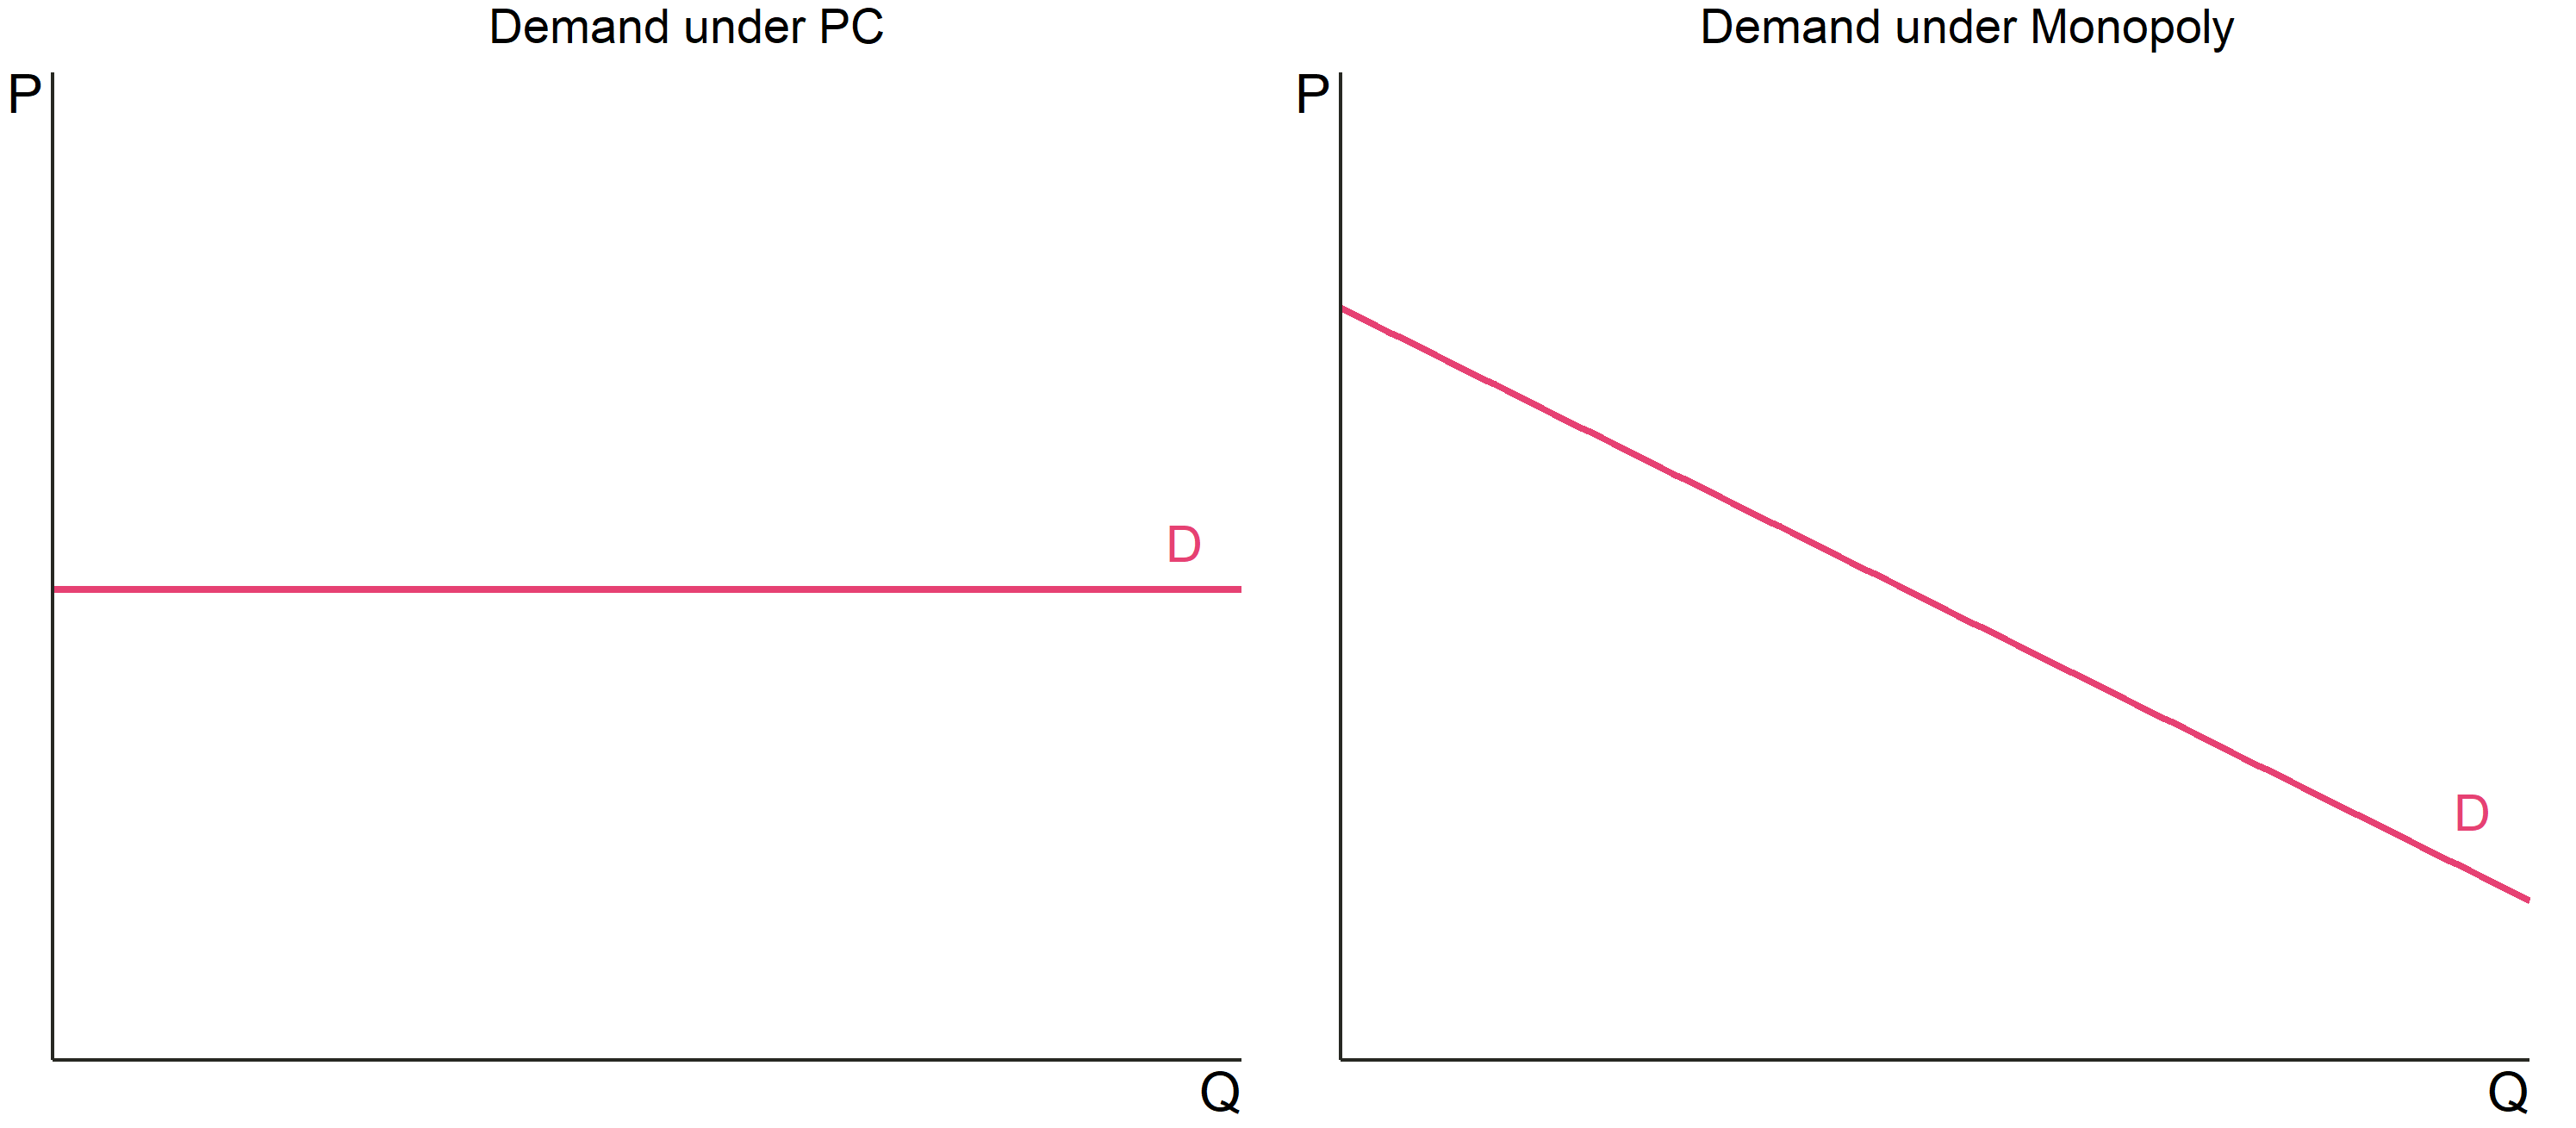
\includegraphics[width=8.5cm]{D compare.png}
		\end{figure}
	\end{itemize}
\end{frame}

\begin{frame}{MR Under A Monopoly}
	\begin{itemize}[<+->]
			\item Since monopolists are price makers, and price according to demand, they face a normal, downward facing demand curve
			\item That is, even though the next unit sold gets the monopolist some revenue $P'$, that new price is likely lower than some previous price $P$
		\begin{itemize}
			\item Thus, we get the following result: \textit{For a monopolist, $MR$ is less than the current price of the good}
		\end{itemize} 
		\item In fact: Under a linear demand curve, MR for the monopolist is the same equation for demand, but with twice the slope\footnote{This comes from calculus, but the book provides you with an example table to motivate this (15-2b)}
	\end{itemize}
\end{frame}


\begin{frame}{Demand and MR Under Monopoly}
	\begin{itemize}[<+->]
		\item Our demand curves in monopoly will almost always be linear, generating the following picture:
		\begin{figure}
			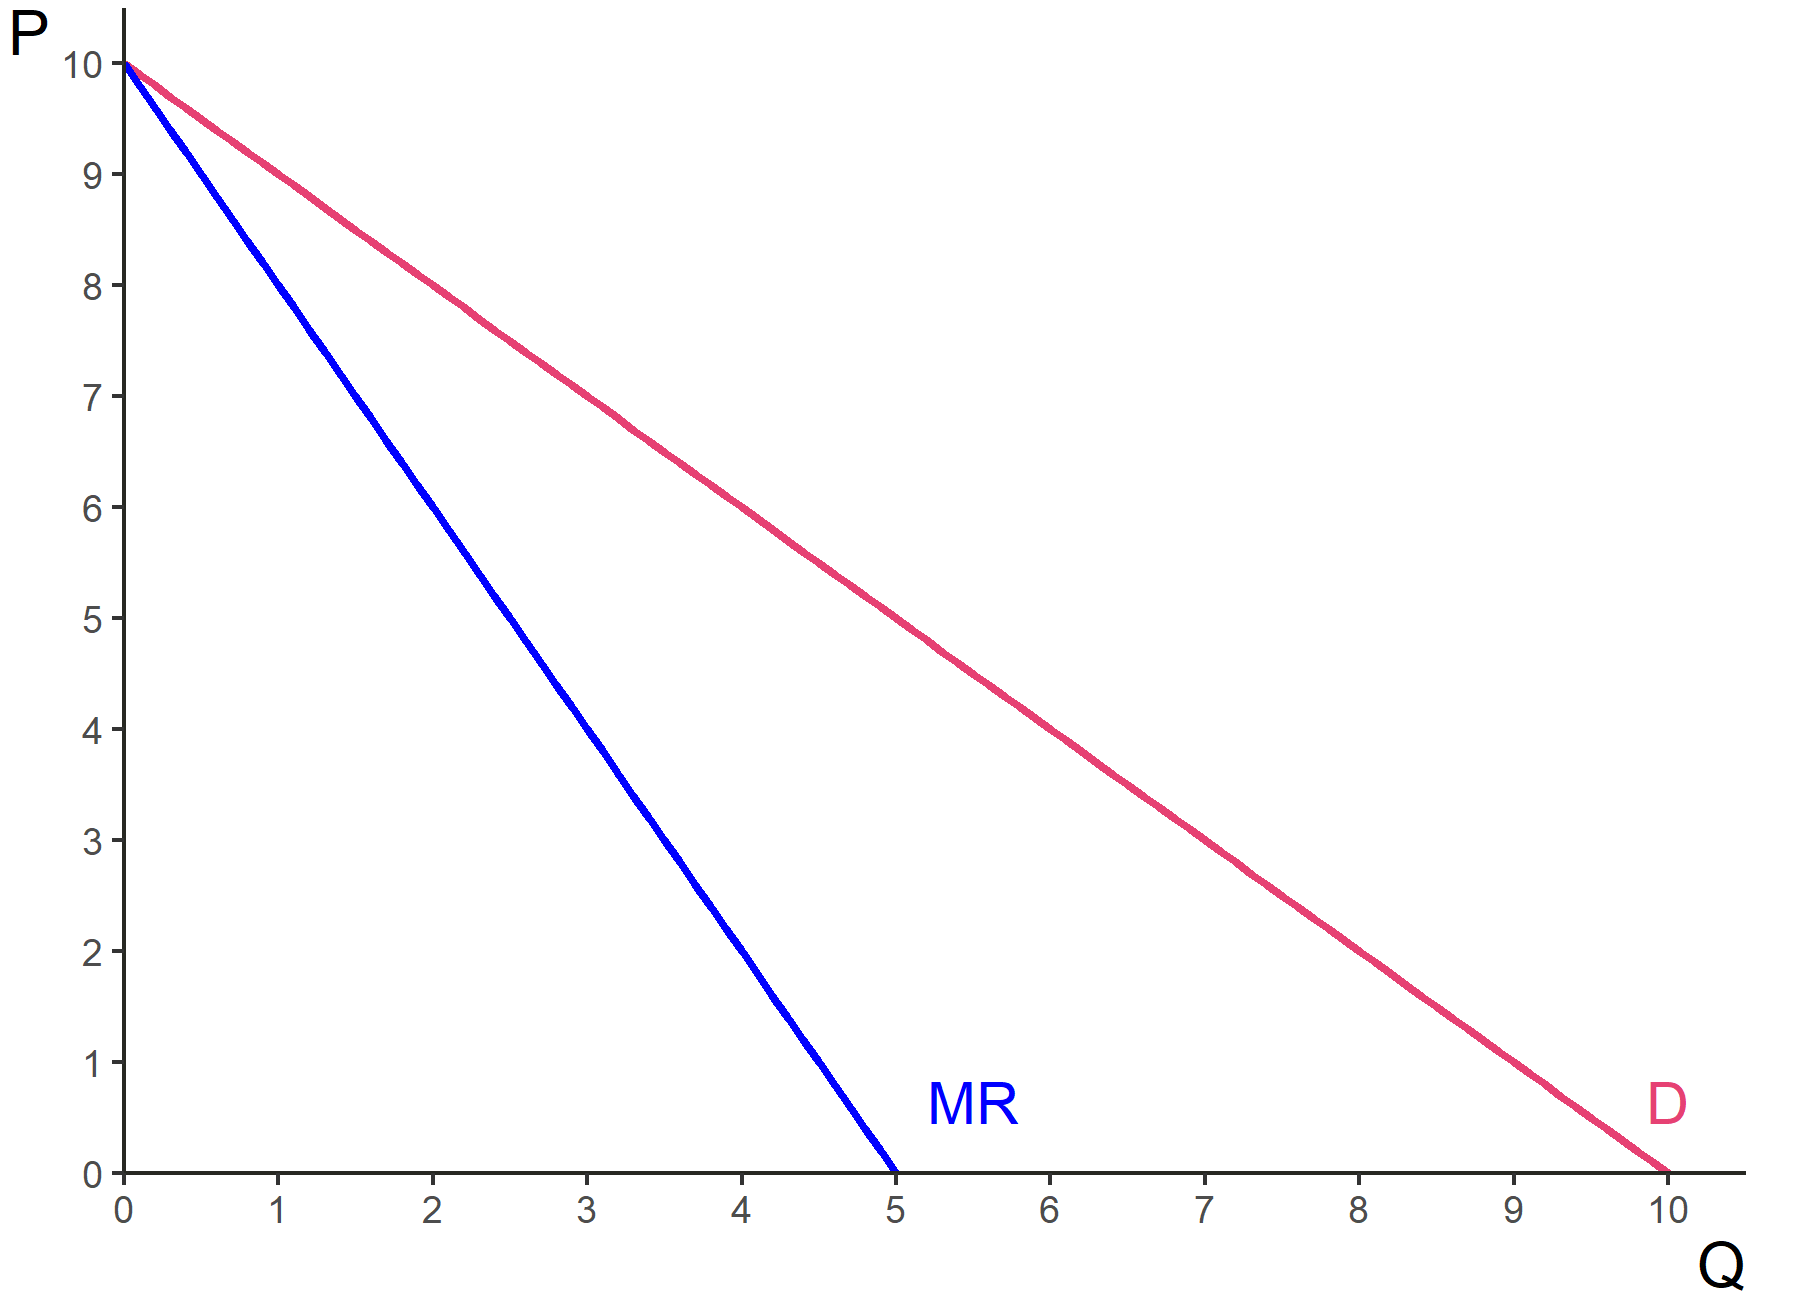
\includegraphics[width=7cm]{mr and d.png}
			%\caption{}
		\end{figure}
		\item That is, the $y-$ intercept is the same, the MR curve just has a slope that is twice as steep
	\end{itemize}
\end{frame}



\begin{frame}{Exercise: Find the Marginal Revenue Curve}
	\begin{itemize}[<+->]
		\item Given the following demand curve, what is marginal revenue?
		
		\item Note that marginal revenue can be negative: this is the price effect overtaking the output effect
	\end{itemize}
\end{frame}

\section*{Profit Maximization Picture}

\begin{frame}{Drawing Pictures in a Monopoly}
	\begin{itemize}[<+->]
		\item In a PC market, we had to draw sets of graphs: one for the market and one for the firm
		\item Here, we can just do one graph. Why?
		\begin{itemize}
			\item There is one firm in the market $\implies$ the firm composes the whole market
		\end{itemize}
		\item Much like with PC markets though, I want you to know the standard shape of the curves and important parts of the graph
		\item Before we get started, there are a few things to note:
		\begin{enumerate}
			\item We will leave absent the notion of a supply curve for a monopolist
			\begin{itemize}
				\item A supply curve takes $P$ as given an determines $Q_{S}$ \item In a monopoly, demand shapes marginal revenue, which determines the optimal production decision, so it does not make sense to talk about a supply curve in this way
			\end{itemize}
			\item Recall this derivation for profit: $\pi=P\cdot Q-TC$, so factoring out a $Q$ yields 
			$$\pi=(P-\frac{TC}{Q})Q=(P-ATC)Q$$
			\begin{itemize}
				\item Does this change for the monopolist?
				\item No
			\end{itemize}
		\end{enumerate}
	\end{itemize}
\end{frame}


\begin{frame}{Optimal Production for the Monopolist}
	\begin{itemize}[<+->]
		\item To begin, the monopolist chooses to produce where $MR=MC$:
		\begin{figure}
			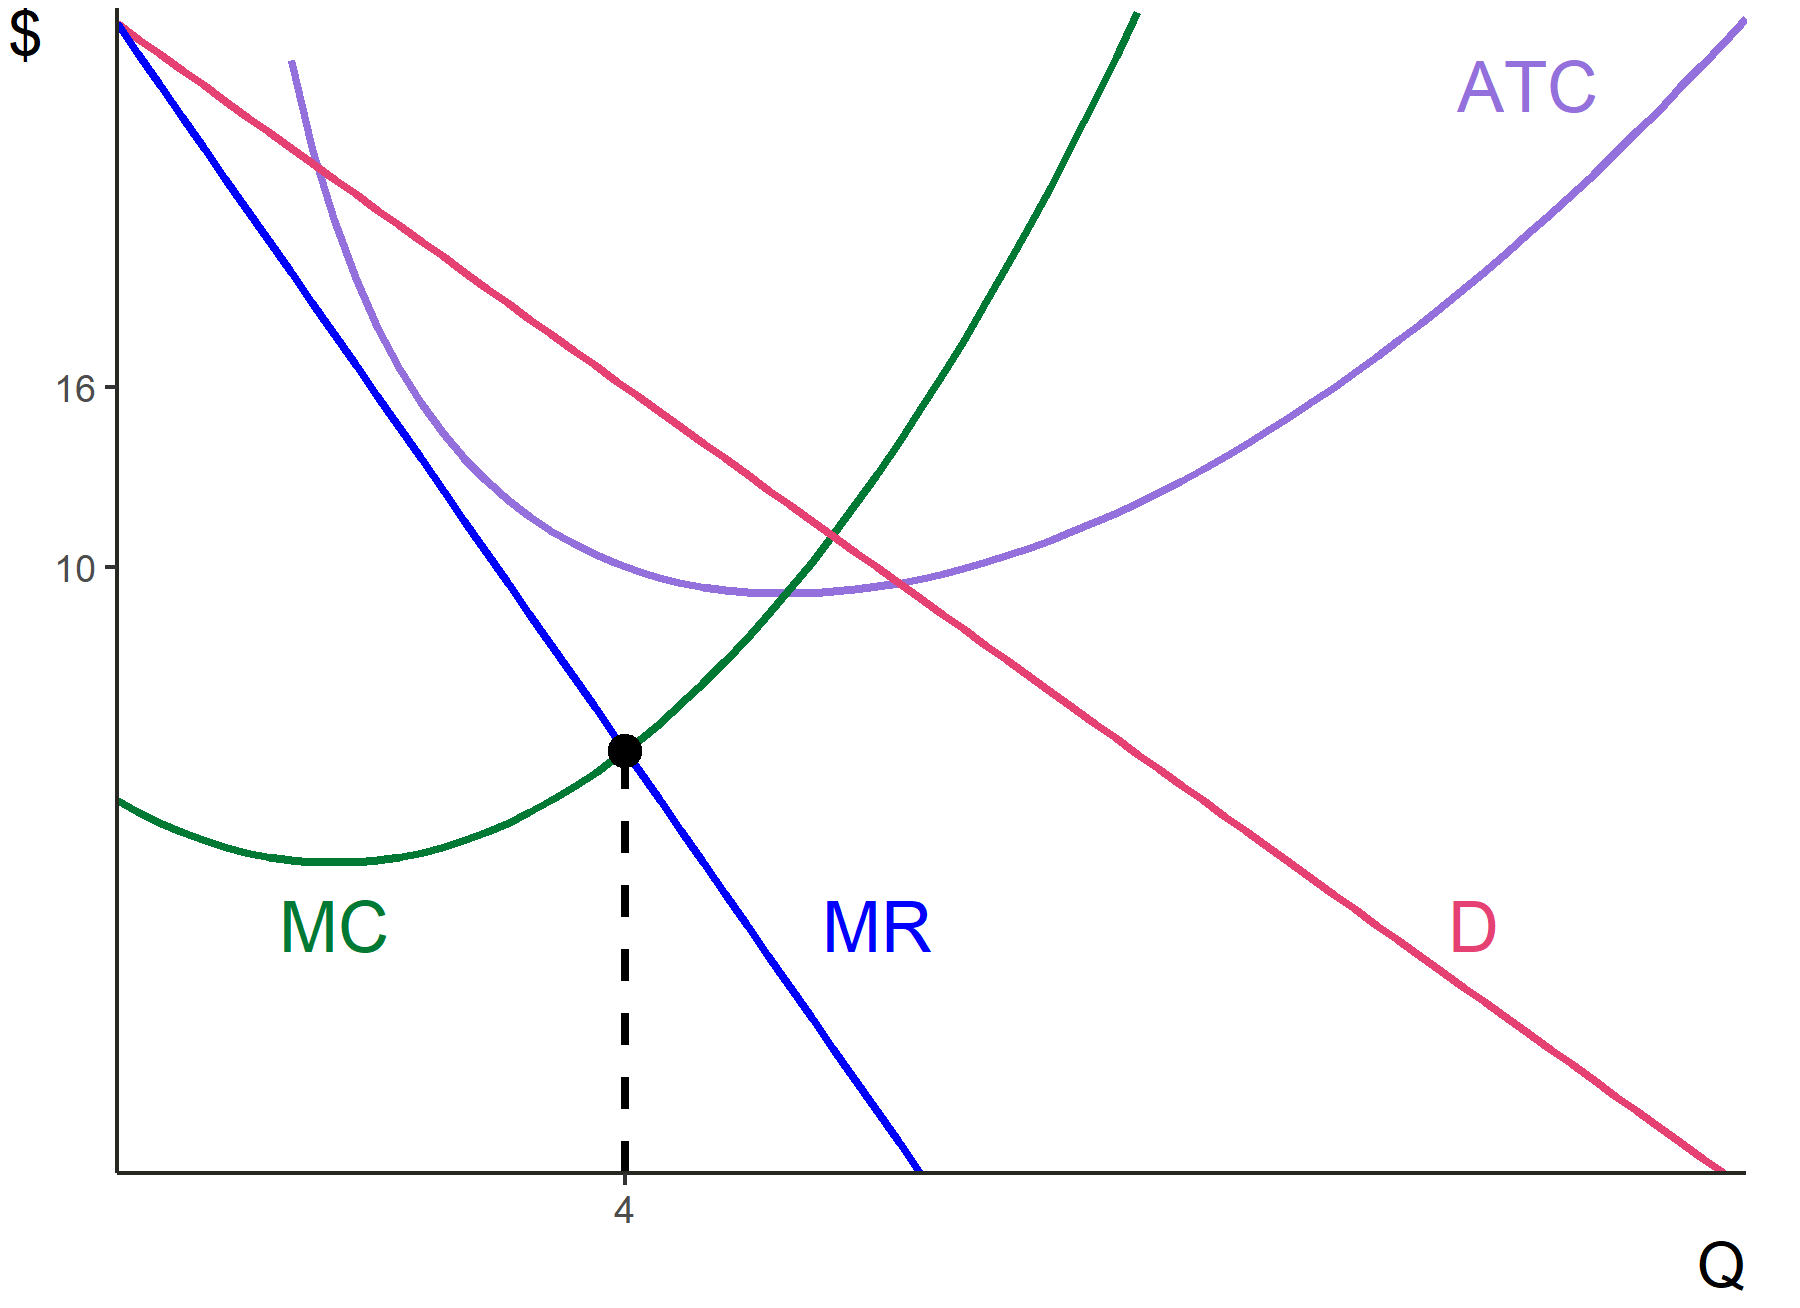
\includegraphics[width=7cm]{mono 1.png}
			\caption*{In this case, the monopolist produces 4 units}
		\end{figure}
	\end{itemize}
\end{frame}

\begin{frame}{Price-Setting for the Monopolist}
	\begin{itemize}[<+->]
		\item The monopolist then charges a price according to the demand schedule, at the level they are producing at:
		\begin{figure}
			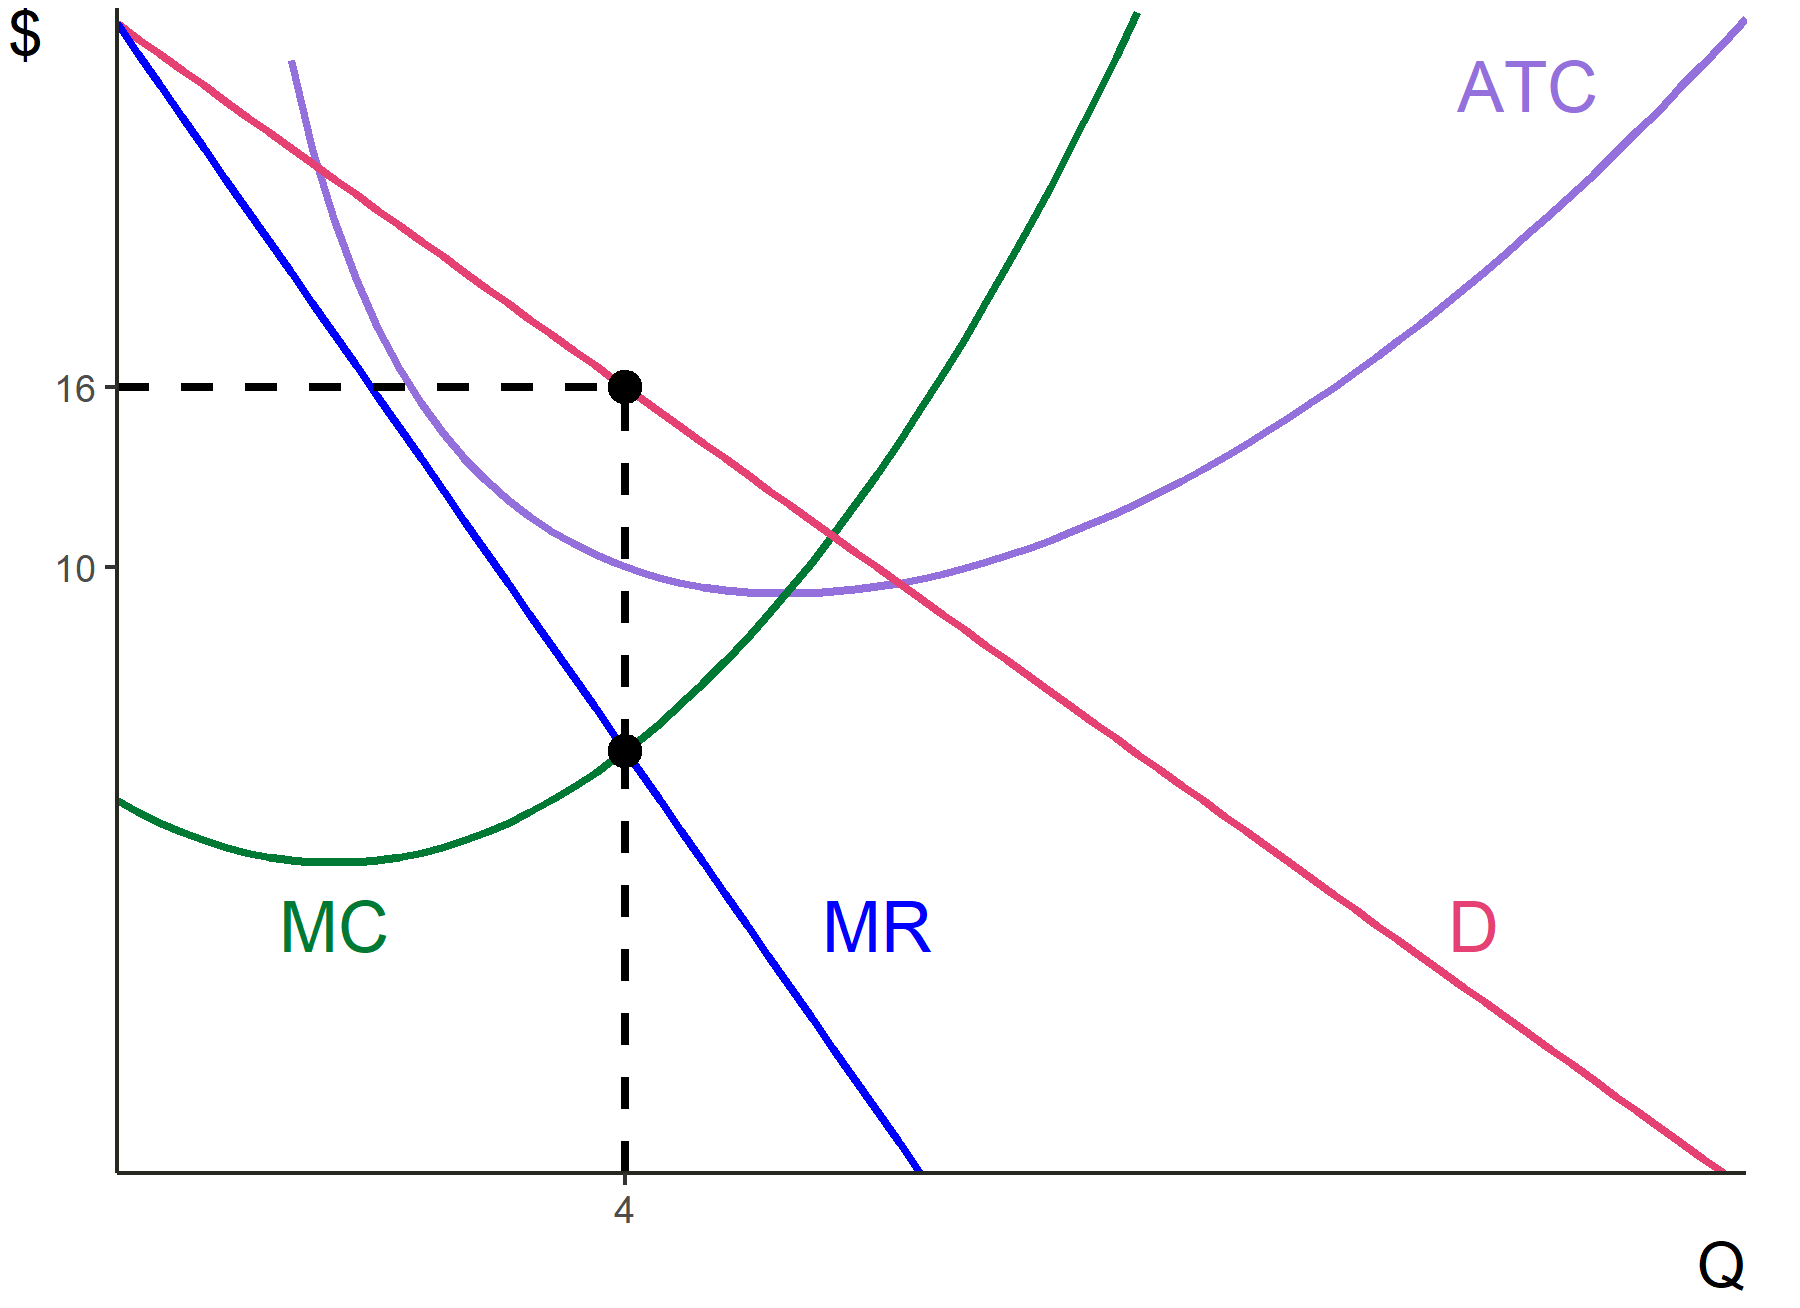
\includegraphics[width=7cm]{mono 2.png}
			\caption*{In this case, a price of $\$16$}
		\end{figure}
	\end{itemize}
\end{frame}

\begin{frame}{Profit for the Monopolist}
	\begin{itemize}[<+->]
		\item The monopolist gets $\pi=(P-ATC)Q$:
		\begin{figure}
			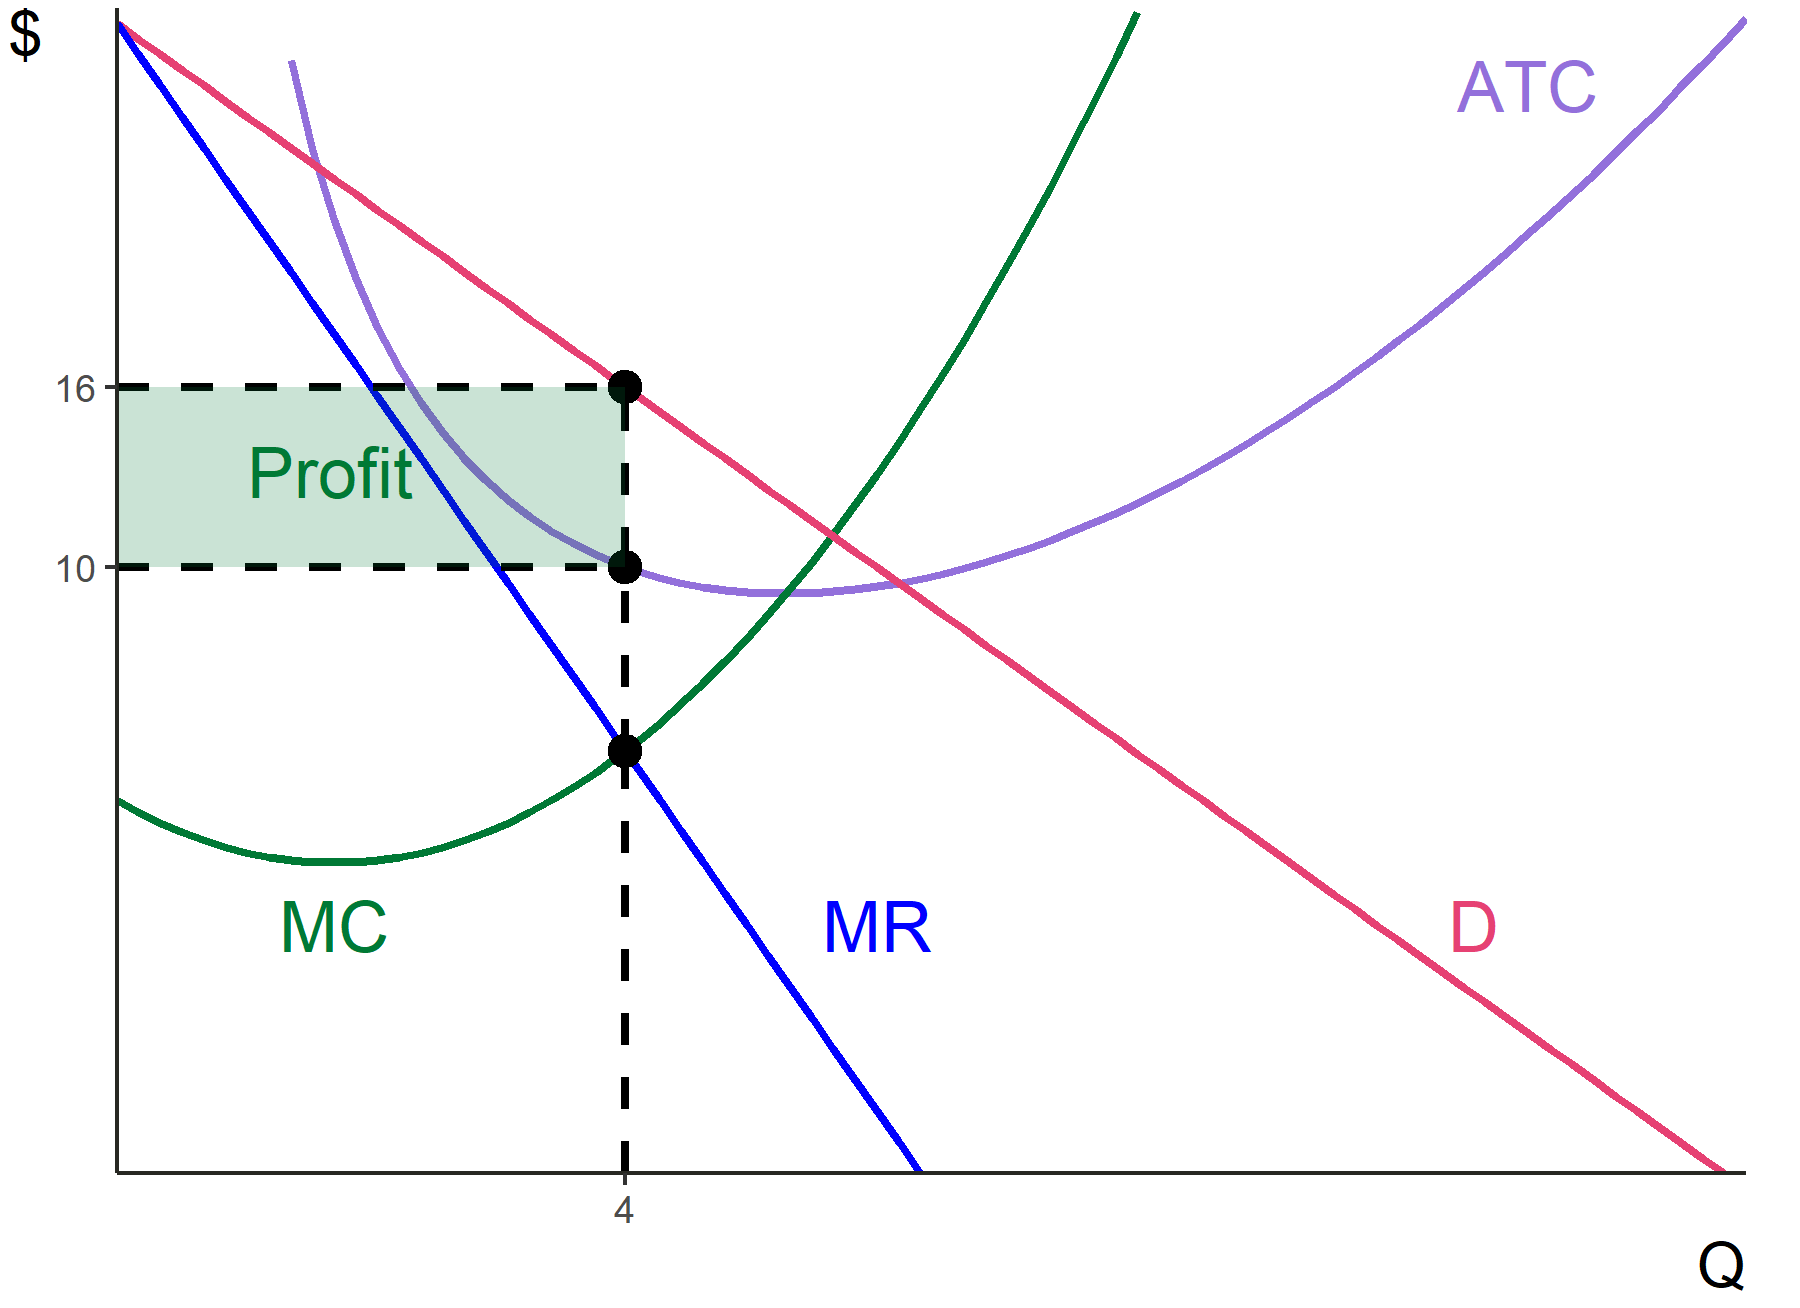
\includegraphics[width=7cm]{mono 3.png}
			\caption*{In this case, a profit of $(16-10)(4)=\$24$}
		\end{figure}
	\end{itemize}
\end{frame}

\begin{frame}{Exercise -- Monopoly Problem}
	\begin{itemize}[<+->]
		\item Determine the optimal production, price-set, and profit by the monopolist. Also determine the marginal cost that the monopolist faces at their optimal level of production.
		\begin{figure}
			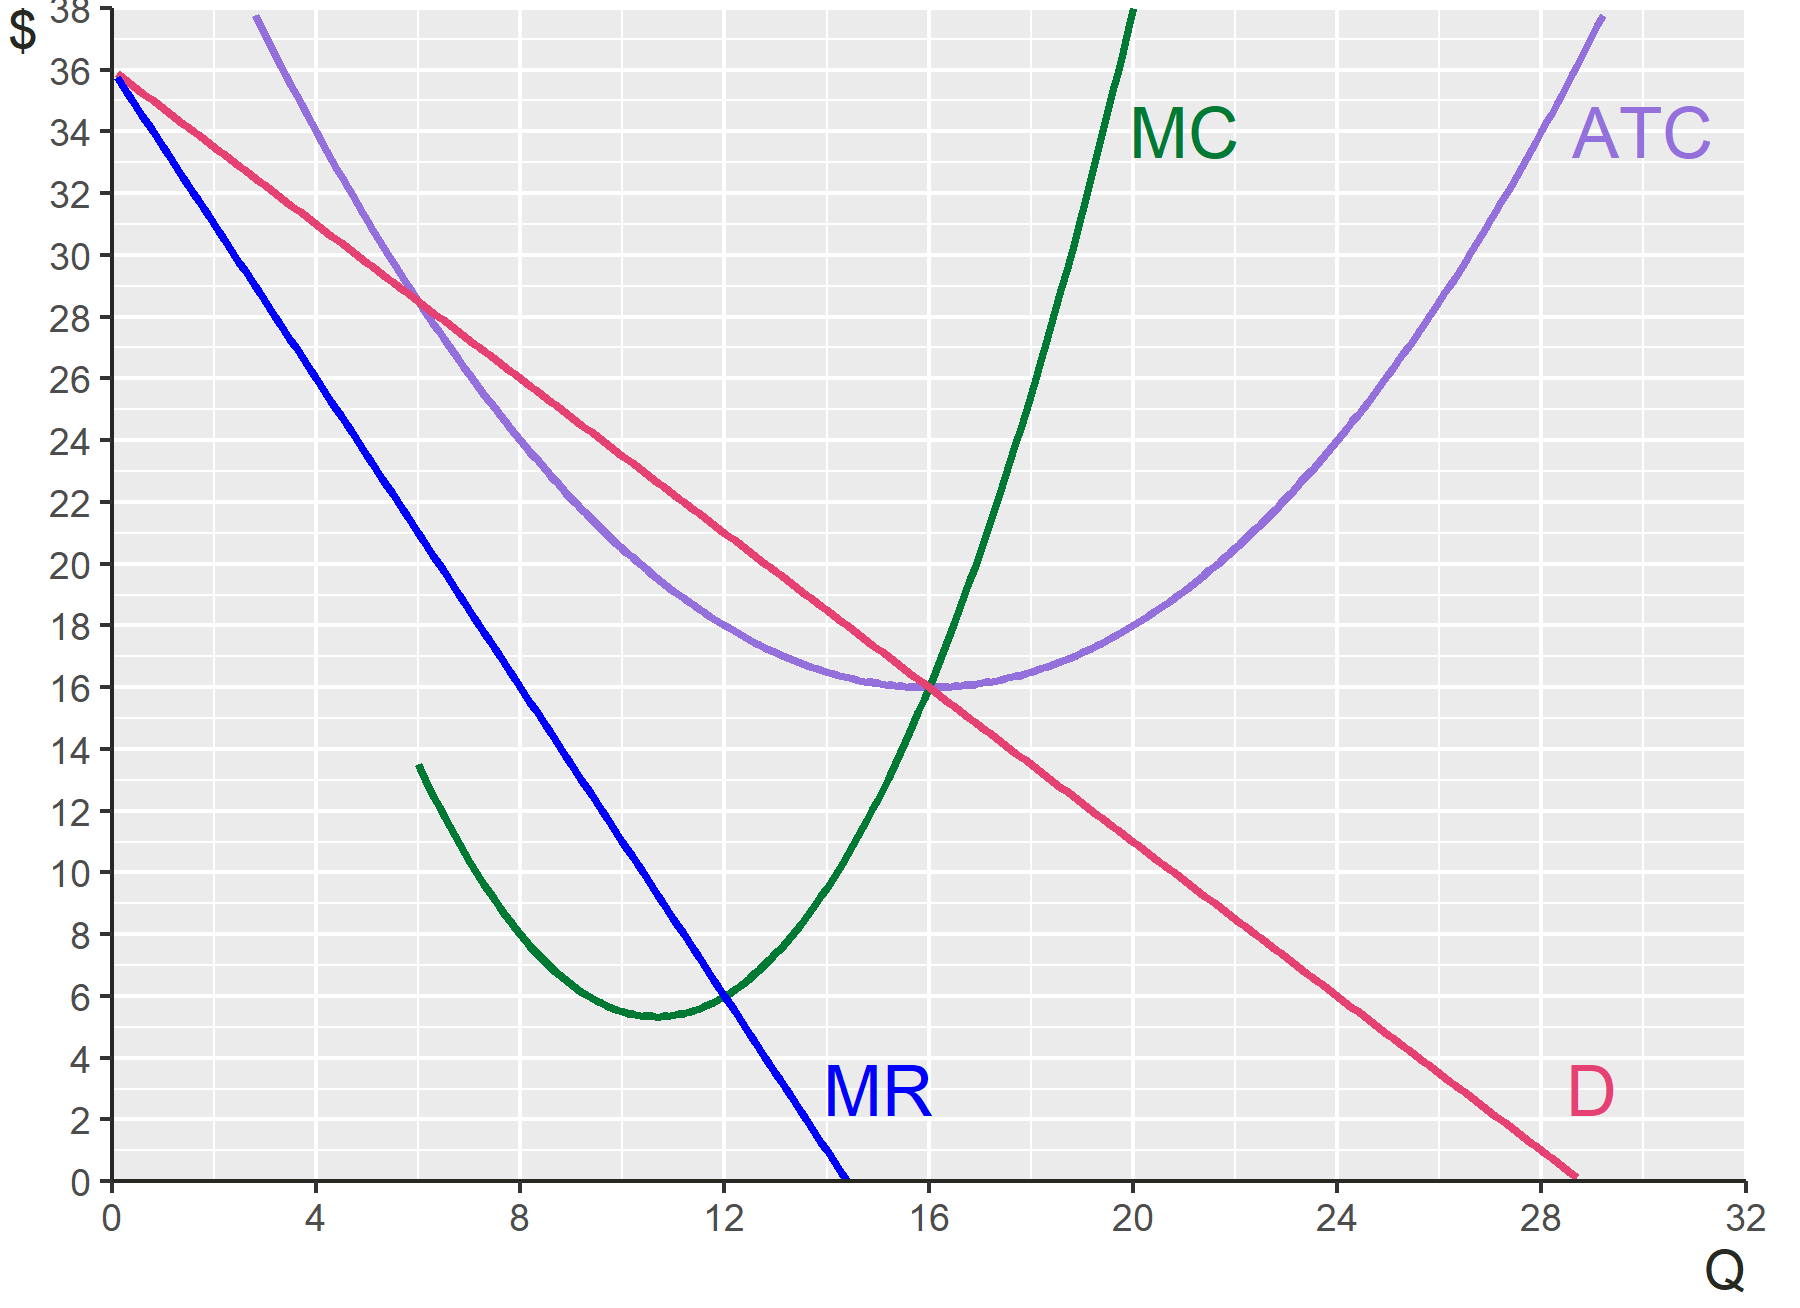
\includegraphics[width=7cm]{mono ex 1.png}
		\end{figure}
	\end{itemize}
\end{frame}

\begin{frame}{Solution -- Monopoly Problem}
	\begin{itemize}[<+->]
		\item The monopolist makes 12 units, for a marginal cost of $\$6$
		\begin{figure}
			\includegraphics<1>[width=7cm]{mono ex 2.png}
			\includegraphics<2>[width=7cm]{mono ex 3.png}
		\end{figure}
	\item<2-> The monopolist sets a price of $\$21$, and makes $(21-18)(12)=\$36$ in profit
	\end{itemize}
\end{frame}


\begin{frame}{Shutdown for Monopoly}
	\begin{itemize}[<+->]
		\item As aforementioned, we will not discuss a monopolists supply curve
		\item For this reason, and because the book doesn't mention it, we will not make a great deal of the monopolist's shutdown condition either
		\item However, for completeness, I did want to discuss it
		\item Recall that we should shut down if the price we are selling for is not covering our variable costs, on average
		\item Now, $P$ is determined by $P(Q)$ in the demand equation
		\item Thus, it might be more accurate to write: \textit{shut down if }
		$$P(Q)<AVC$$
		\item The following picture shows such an example when the monopolist will shut down
	\end{itemize}
\end{frame}

\begin{frame}{Shutdown for Monopoly, Visualized}
	\begin{figure}
		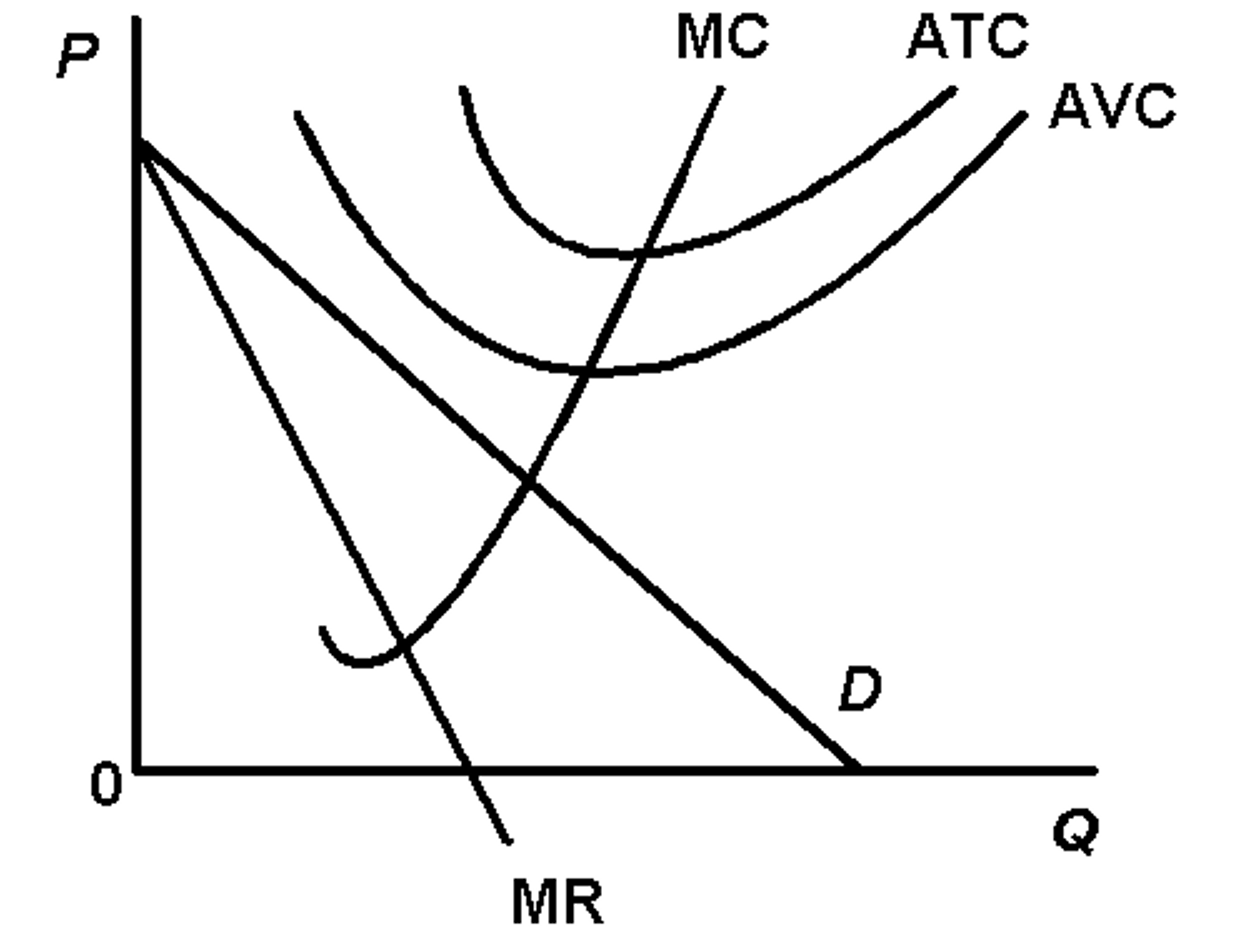
\includegraphics[width = 7cm]{monop shut.png}
	\end{figure}
	\begin{itemize}[<+->]
		\item Of course, if demand at $Q^{*}$ were in between AVC and ATC, the monopolist would operate at a loss in the short run
	\end{itemize}
\end{frame}


\section*{Consequences of a Monopoly}


\begin{frame}{Optimal Production under PC}
	\begin{itemize}[<+->]
		\item Recall the case of perfect competition. Specifically, suppose we have identical perfectly competitive firms, such that the following is the market graph
		\begin{figure}
			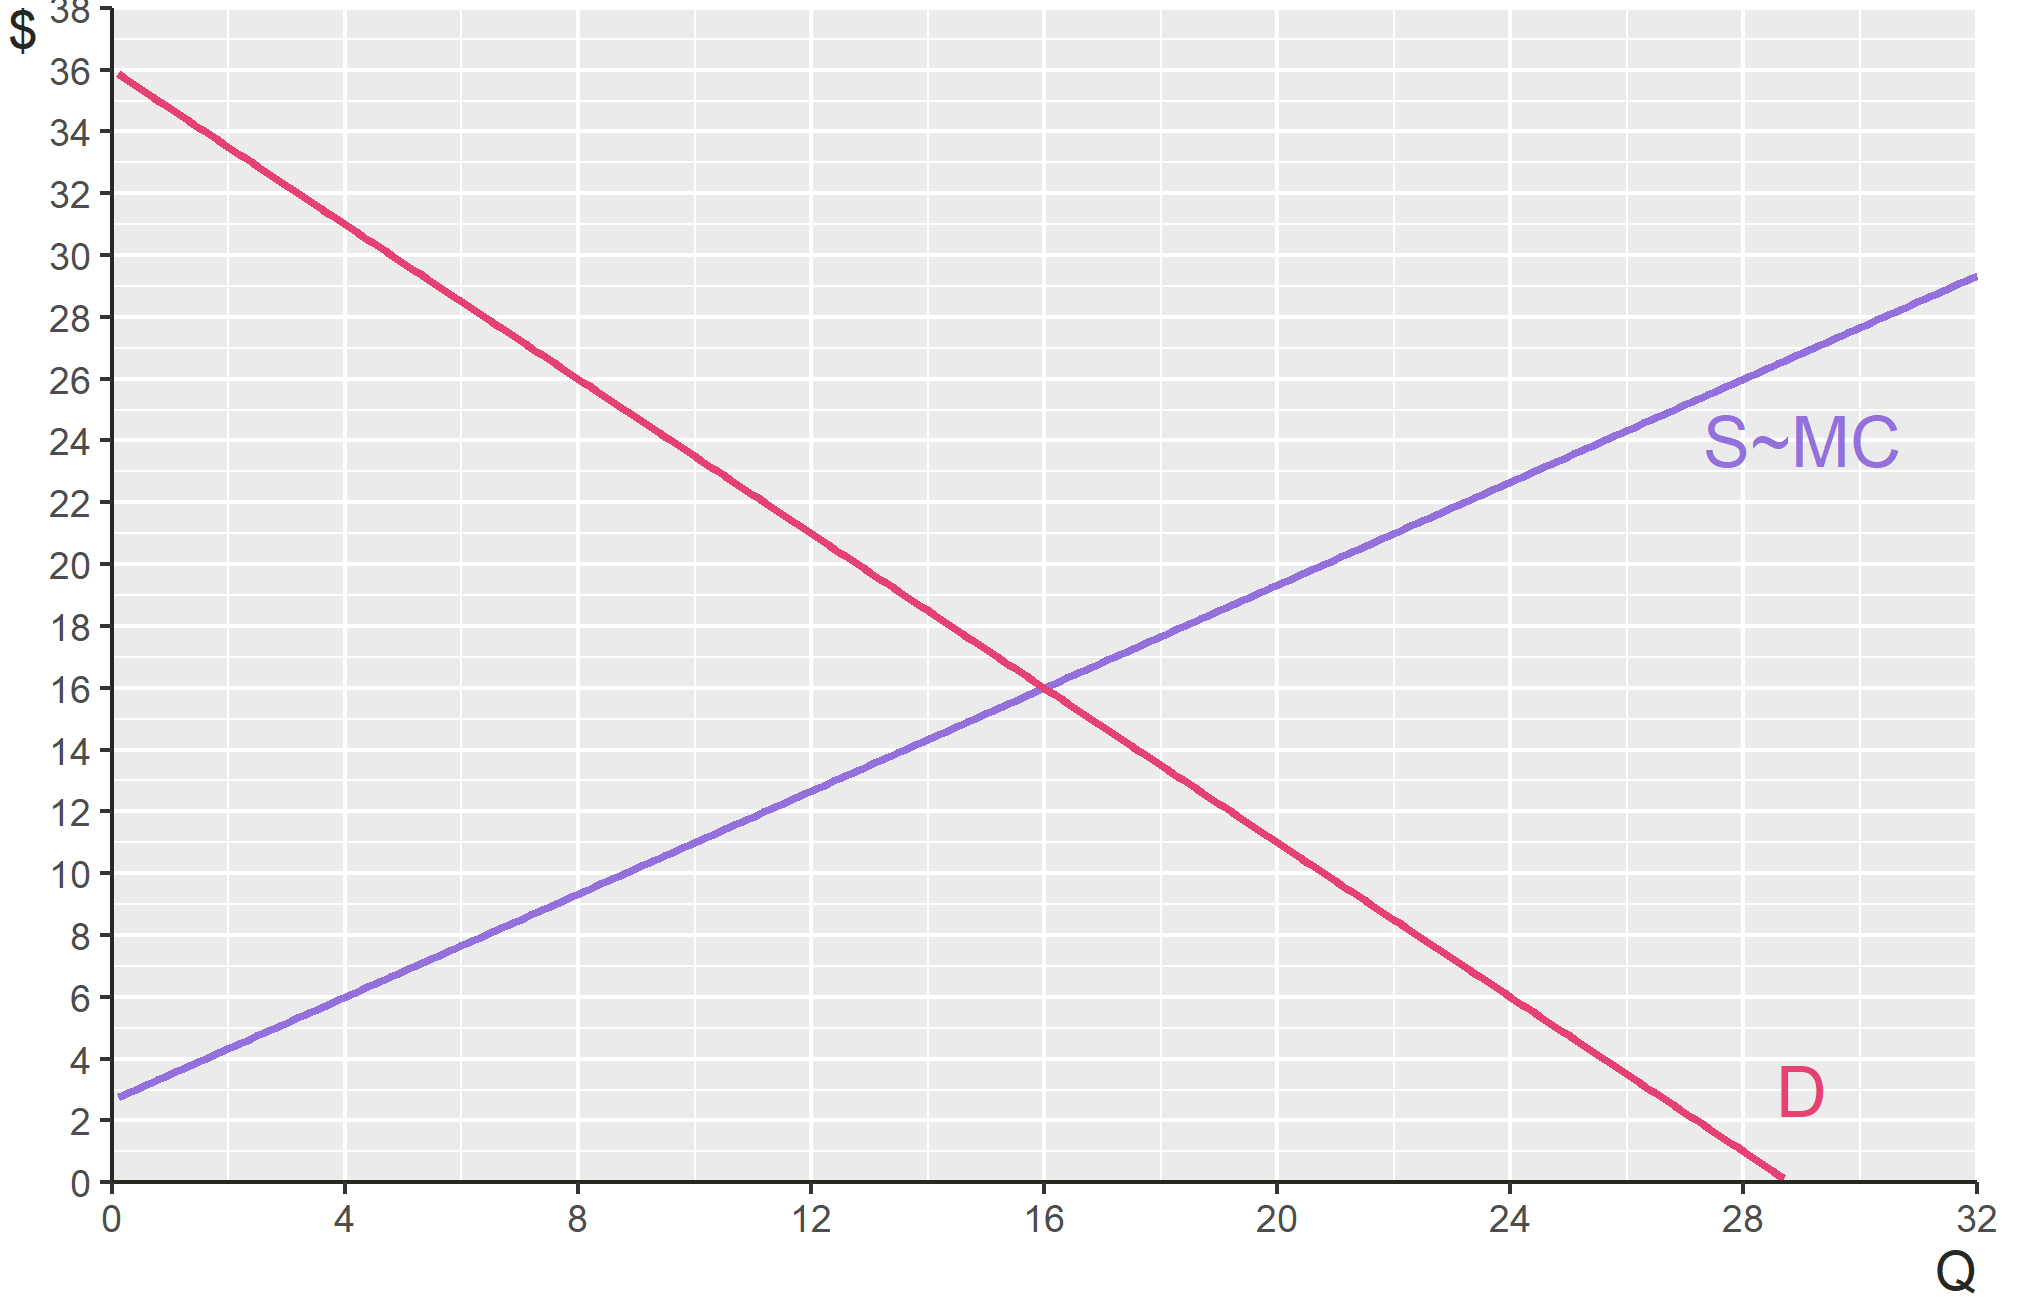
\includegraphics[width=7cm]{pcm 1.png}
			%\caption*{}
		\end{figure}
		\item Short-run supply is a reflection of firms' marginal costs
	\end{itemize}
\end{frame}

\begin{frame}{Optimal Production under PC}
	\begin{itemize}[<+->]
		\item The firm is producing where $S=D$, with $Q^{*}=16$ and $P^{*}=16$ as well
		\begin{figure}
			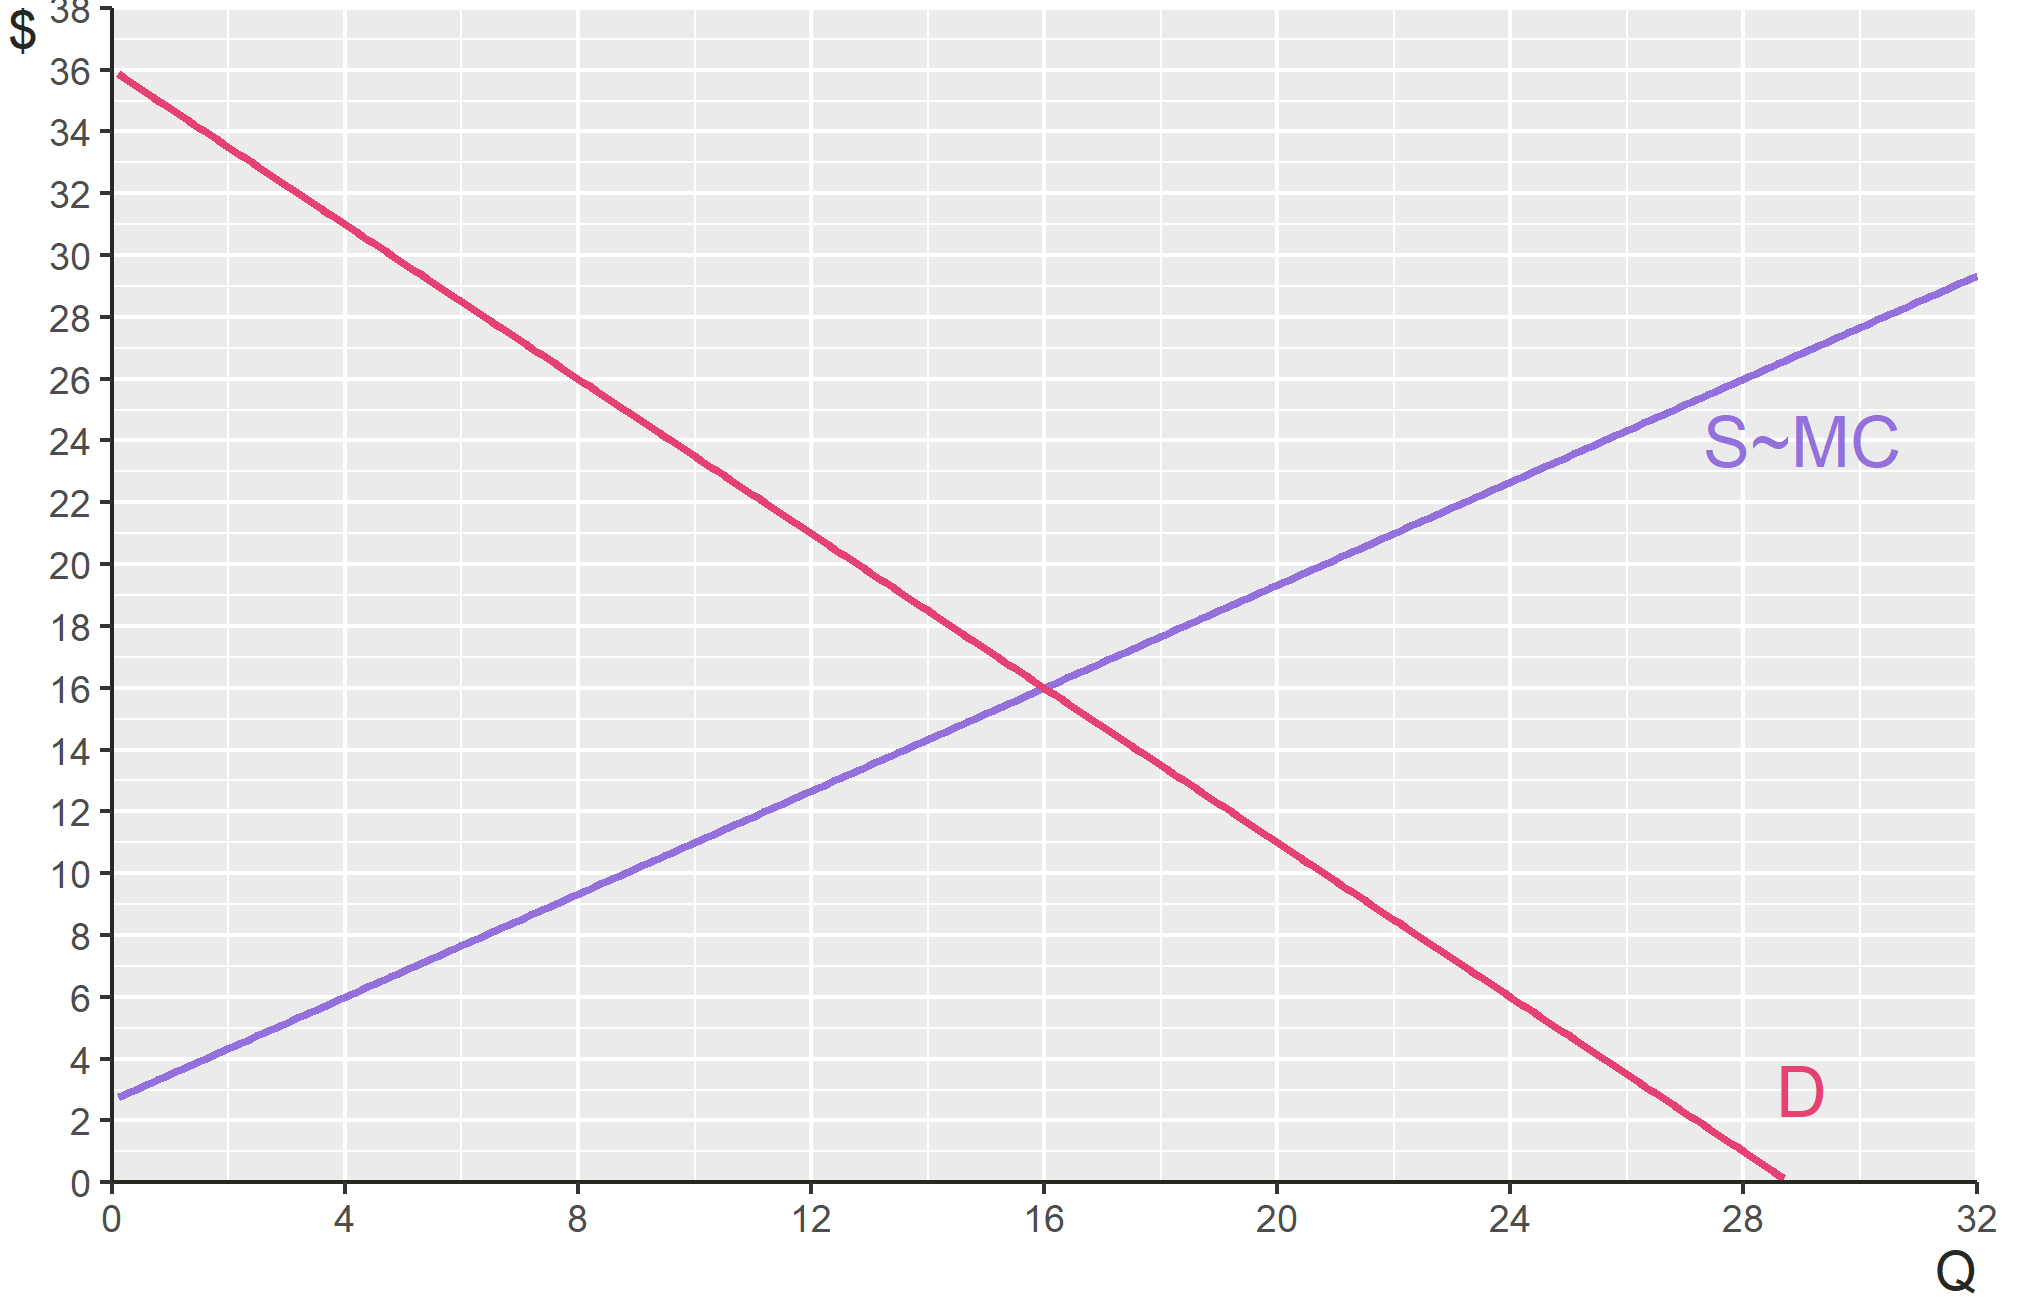
\includegraphics[width=7cm]{pcm 1.png}
			%\caption*{}
		\end{figure}
		\item Recall that the PC firm is making 0 profit in the long run
	\end{itemize}
\end{frame}

\begin{frame}{TS under PC}
	\begin{itemize}[<+->]
		\item Finally, TS is given by 
		\begin{figure}
			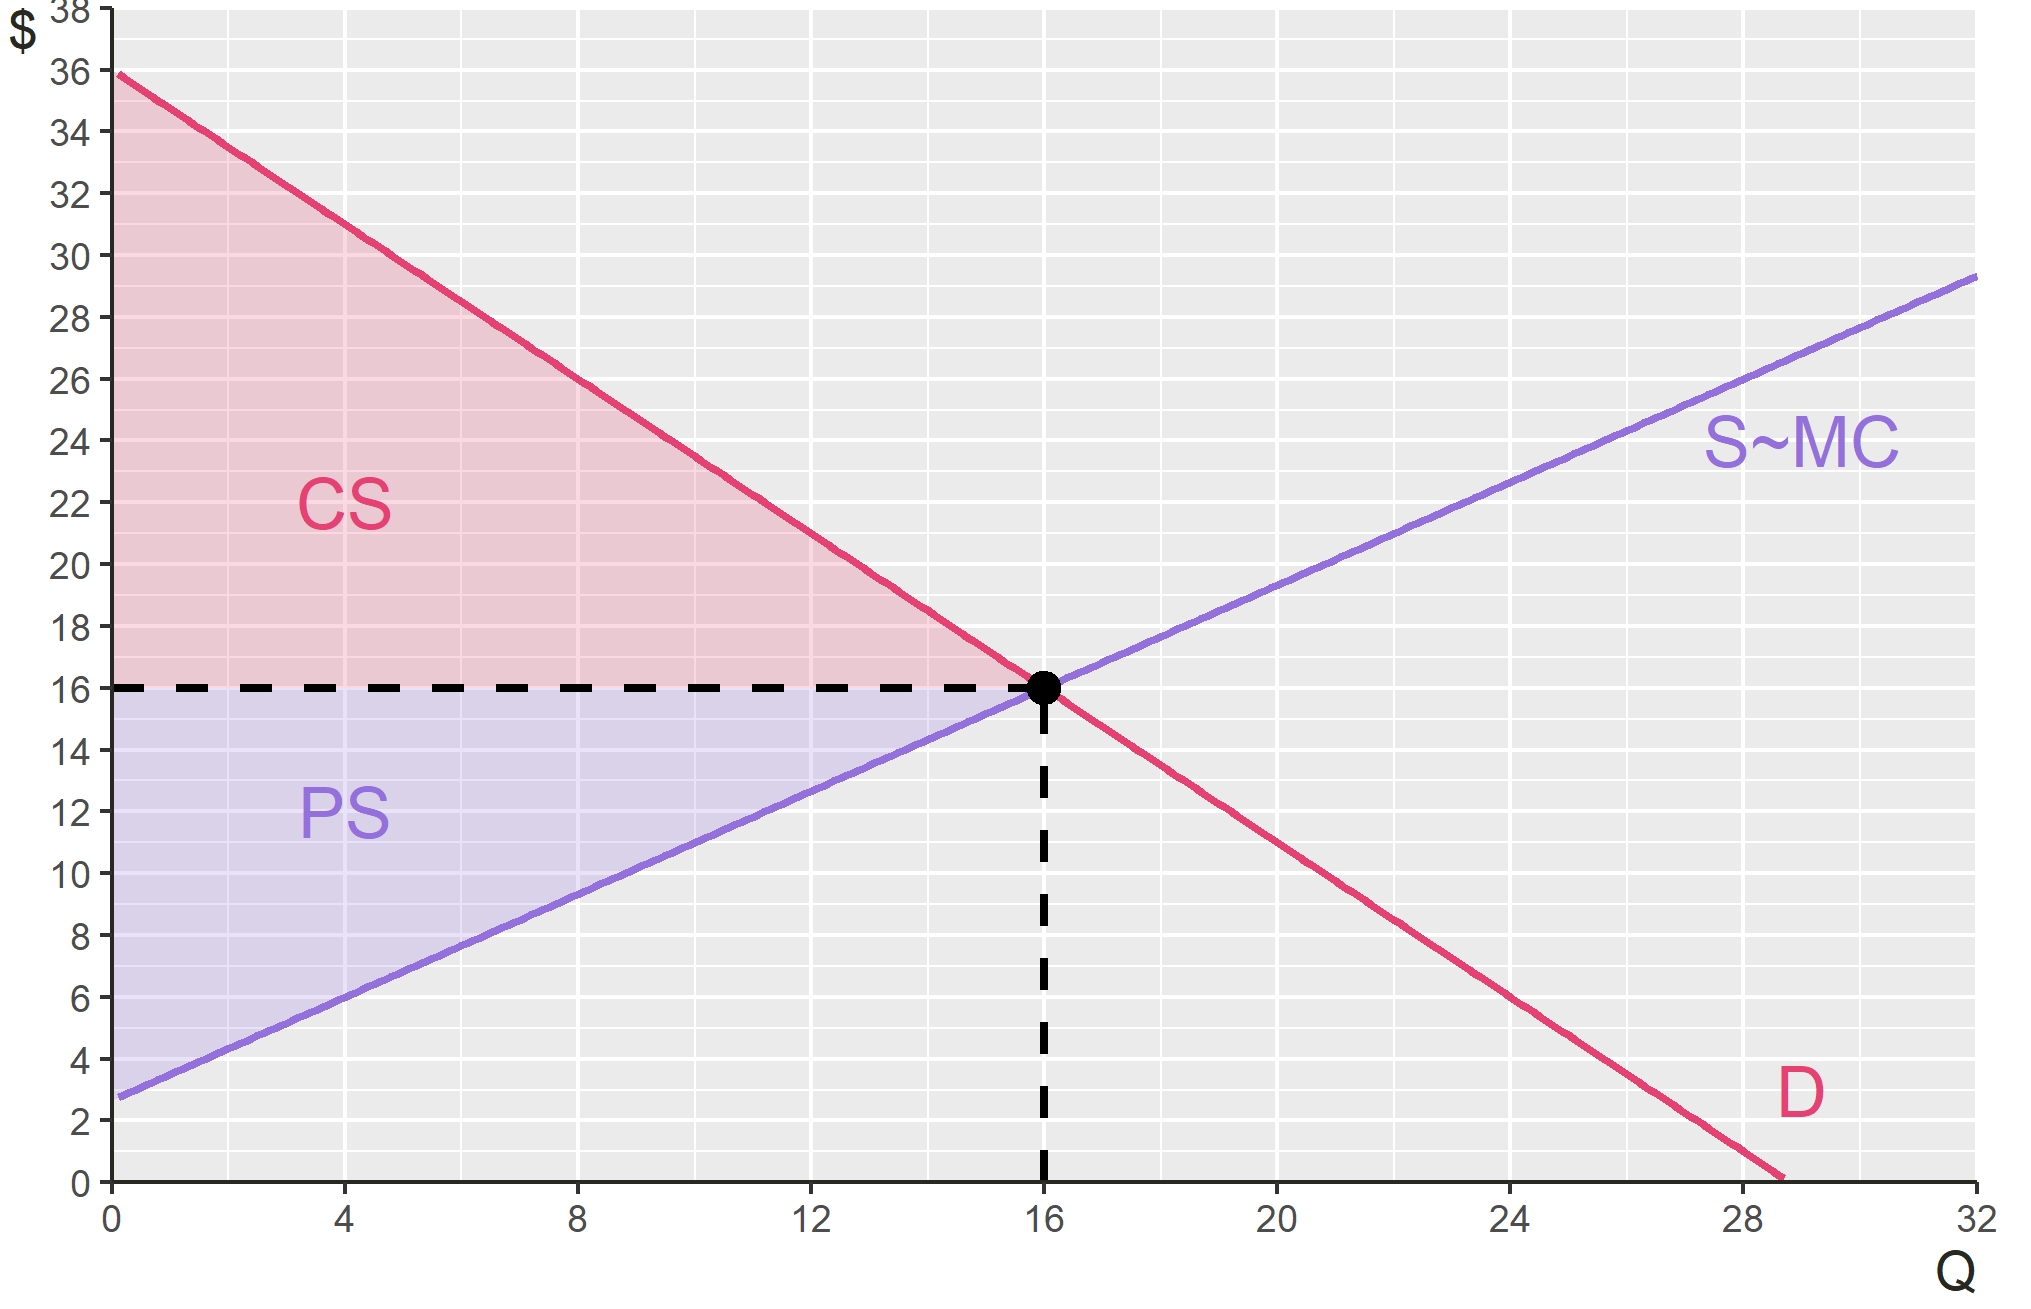
\includegraphics[width=7cm]{pcm 2.png}
			%\caption*{}
		\end{figure}
		\item In this case, $TS=\frac{1}{2}(36-16)(16)+\frac{1}{2}(16-\frac{8}{3})(16)=266.\bar{6}$
	\end{itemize}
\end{frame}

\begin{frame}{Optimal Production under Monopoly}
	\begin{itemize}[<+->]
		\item Now consider a monopoly with the same marginal cost curve, facing the same market demand curve:
		\begin{figure}
		\includegraphics<1>[width=7cm]{pcm 3.png}
		\includegraphics<2>[width=7cm]{pcm 4.png}
	\end{figure}
		\item<2-> In this case, the monopolist produces only $Q=10$ units, but charges a higher price: $P=23.5$
	\end{itemize}
\end{frame}

\begin{frame}{LR Profit under Monopoly}
	\begin{itemize}[<+->]
		\item Note that the monopolist earns $\pi=(23.5-20.5)(10)=\$30$
		\begin{figure}
			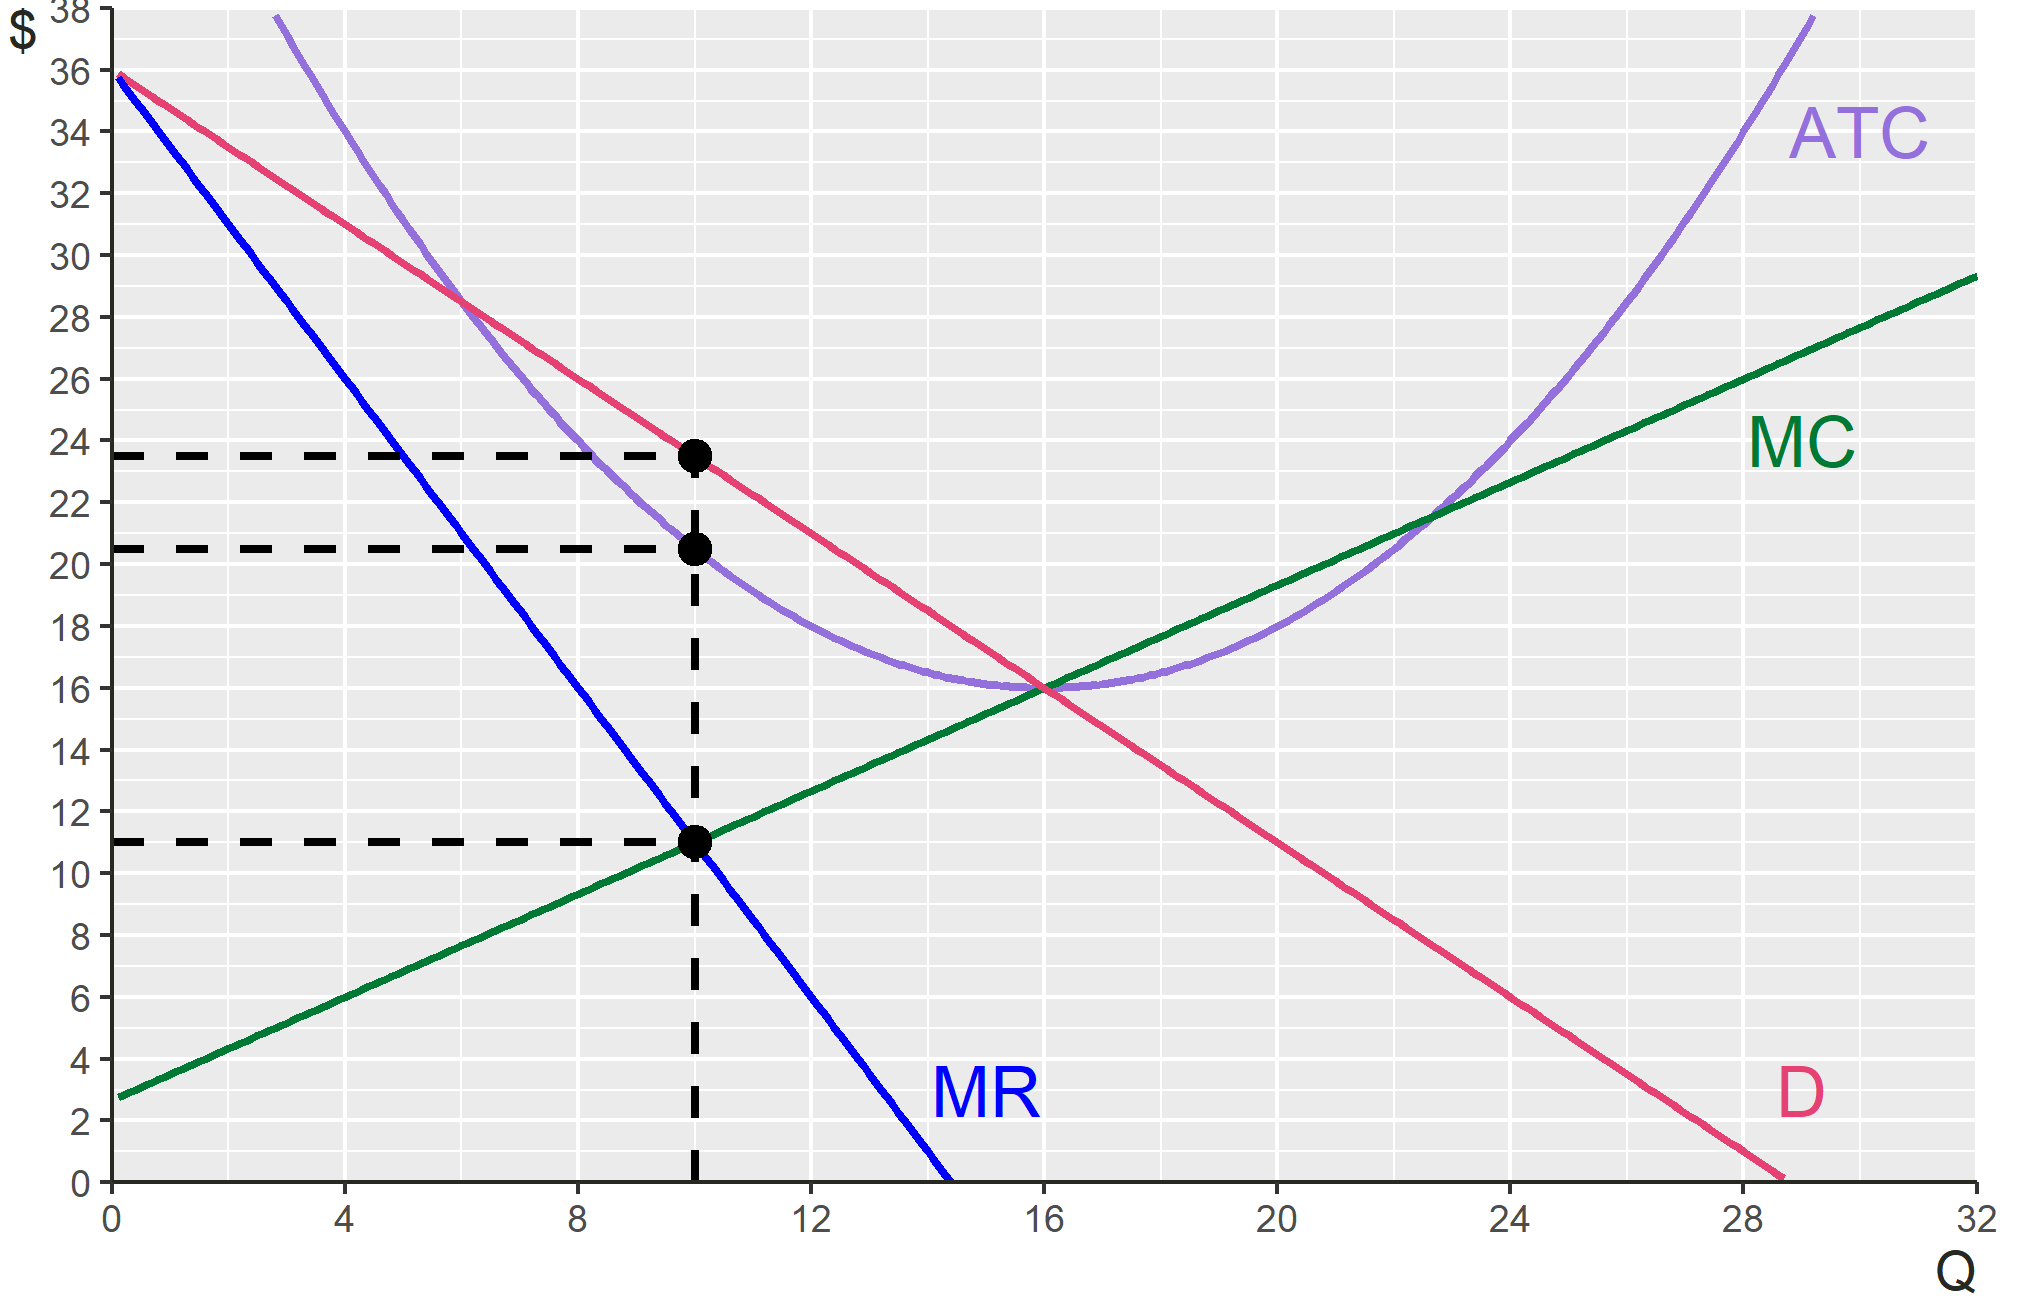
\includegraphics[width=6.5cm]{pcm 4.png}
			%\caption*{}
		\end{figure}
		\item Remember, there are barriers to entry in a monopoly. Therefore, new entry by firms may not be possible (we will generally not consider this possible)
		\item I.e., the monopolist makes positive profit, even in the long run
	\end{itemize}
\end{frame}

\begin{frame}{CS under Monopoly}
	\begin{itemize}[<+->]
		\item Remember: CS is the difference between what willingness to pay, and what consumers actually pay:
		\begin{figure}
			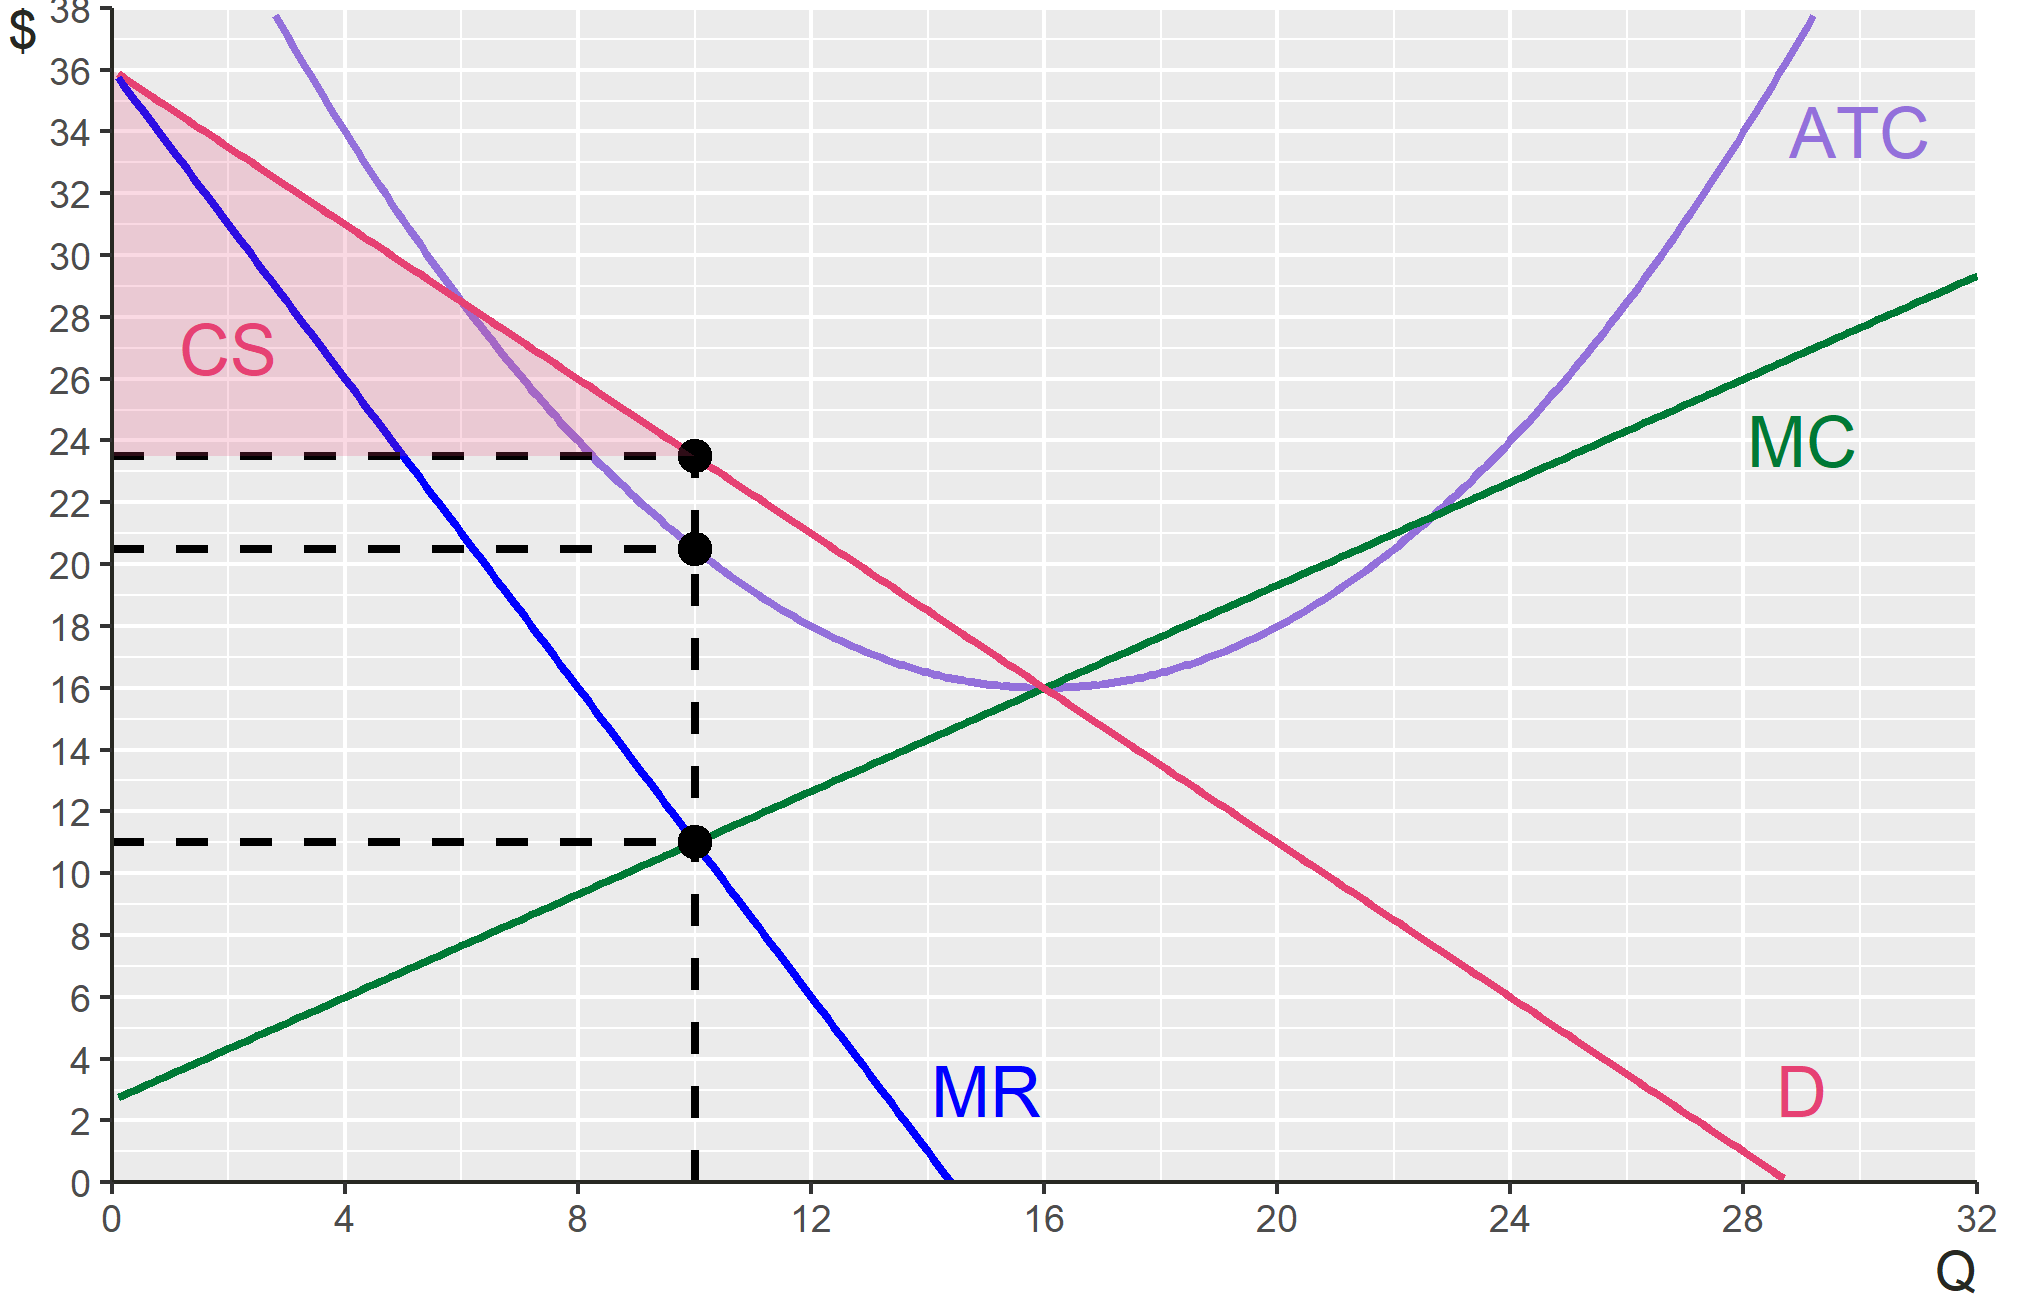
\includegraphics[width=7cm]{pcm 5.png}
			%\caption*{}
		\end{figure}
		\item In this case, $CS=\frac{1}{2}(36-23.5)(10)=62.5$
	\end{itemize}
\end{frame}

\begin{frame}{PS under Monopoly}
	\begin{itemize}[<+->]
		\item Even though we do not have a "supply" curve for the monopolist, we will pretend that $MC$ works just as well
		\begin{itemize}
			\item Given a demand and thereby a MR curve, MC is a reflection of willingness to accept, so this is fine
		\end{itemize}
		\begin{figure}
			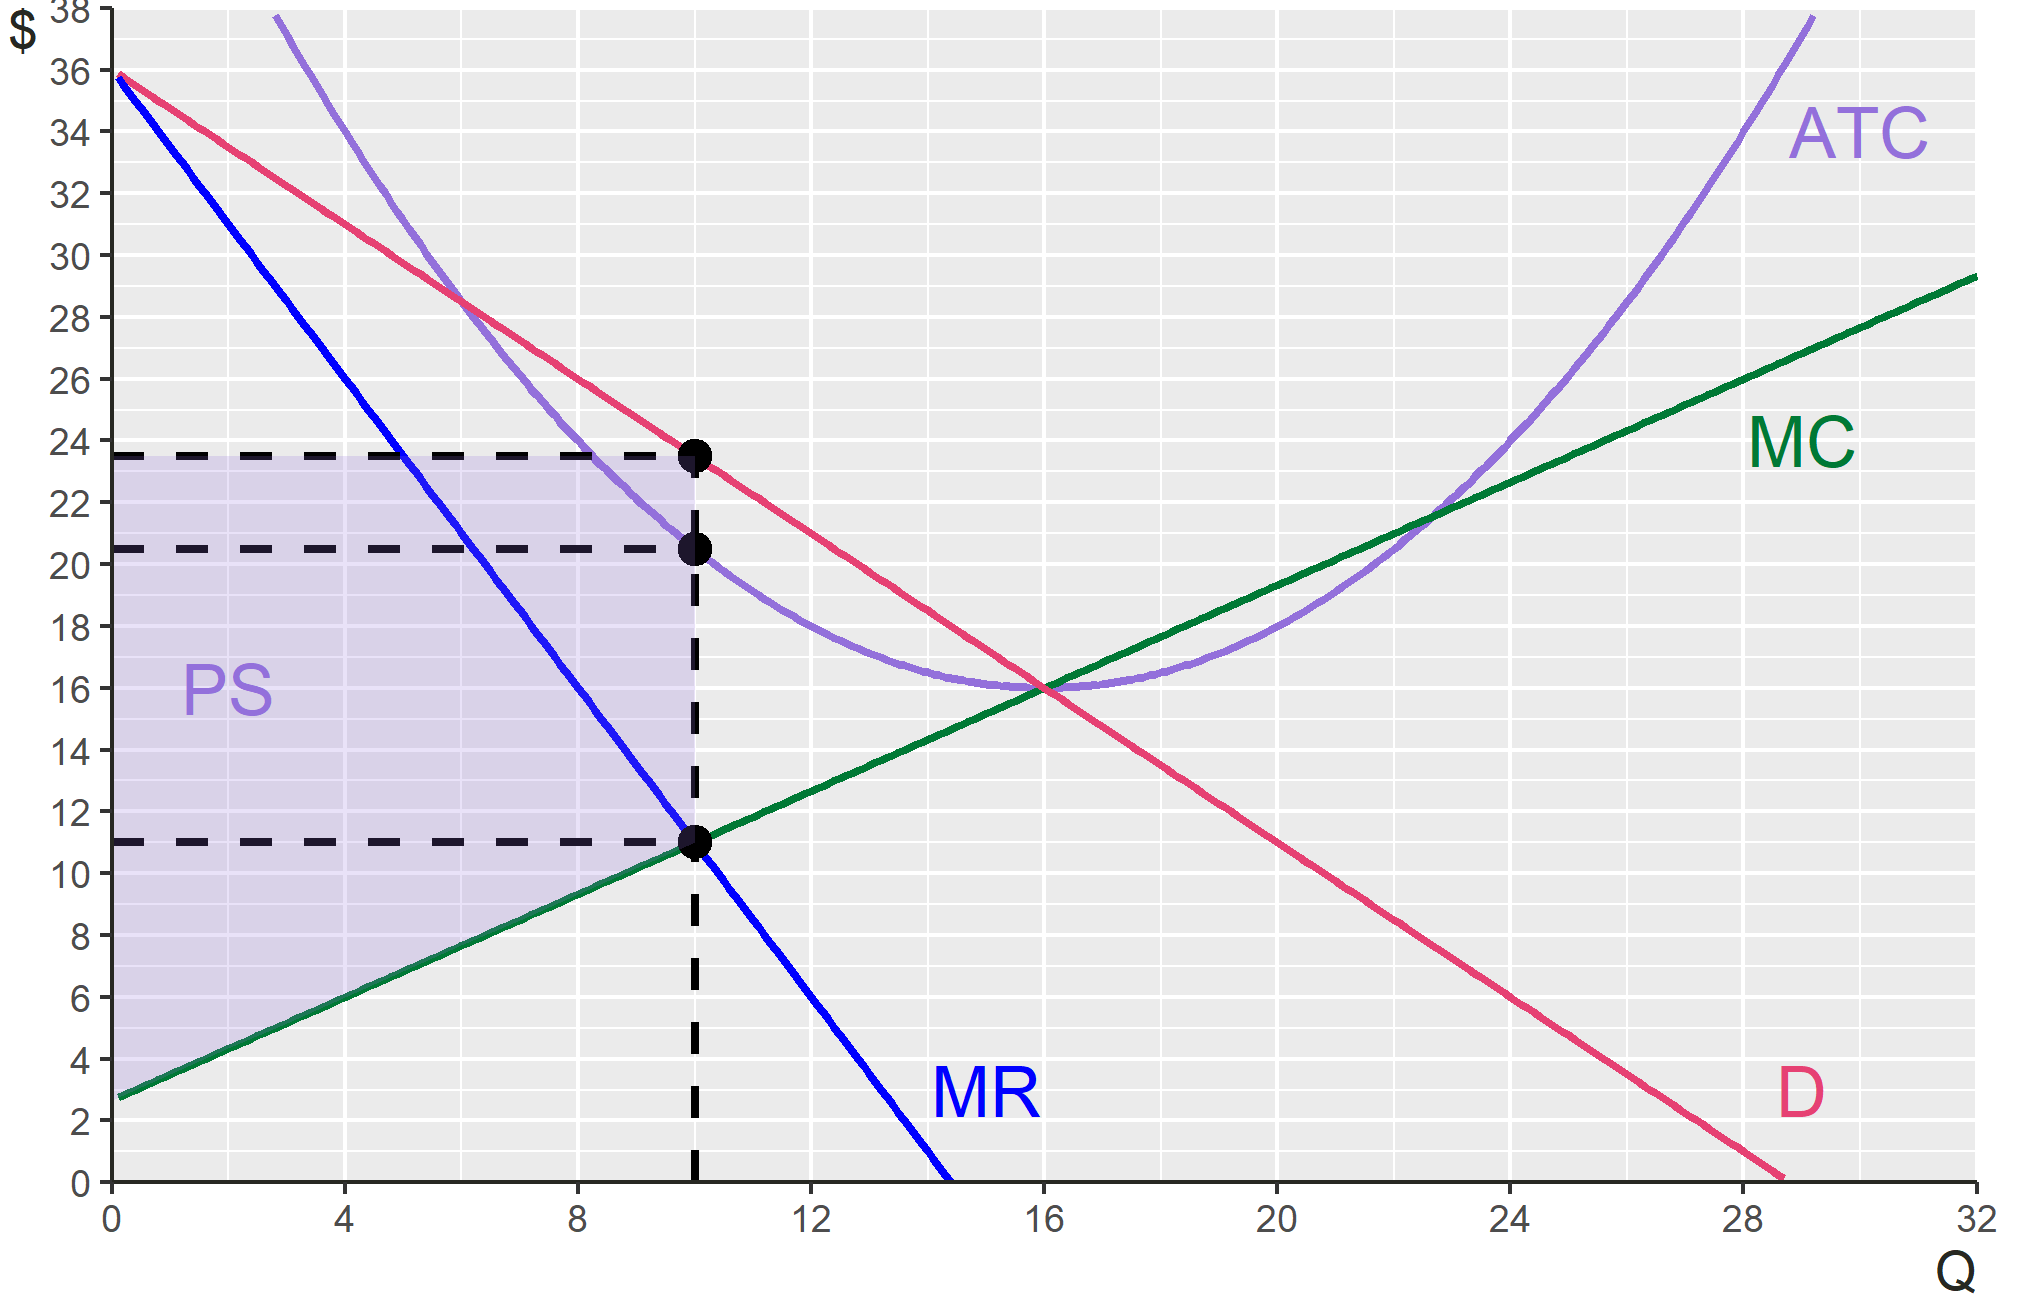
\includegraphics[width=7cm]{pcm 6.png}
			%\caption*{}
		\end{figure}
		\item PS, the difference between price received and WTA, is given by $PS=(23.5-11)(10) + \frac{1}{2}(11-\frac{8}{3})(10)=166.\bar{6}$
	\end{itemize}
\end{frame}

\begin{frame}{TS under Monopoly}
	\begin{itemize}[<+->]
		\item Therefore, TS under monopoly is given by $229.1\bar{6}$
		\item Under PC, it was $266.\bar{6}$
		\item Thus, we have the following DWL under a monopoly:
		\begin{figure}
			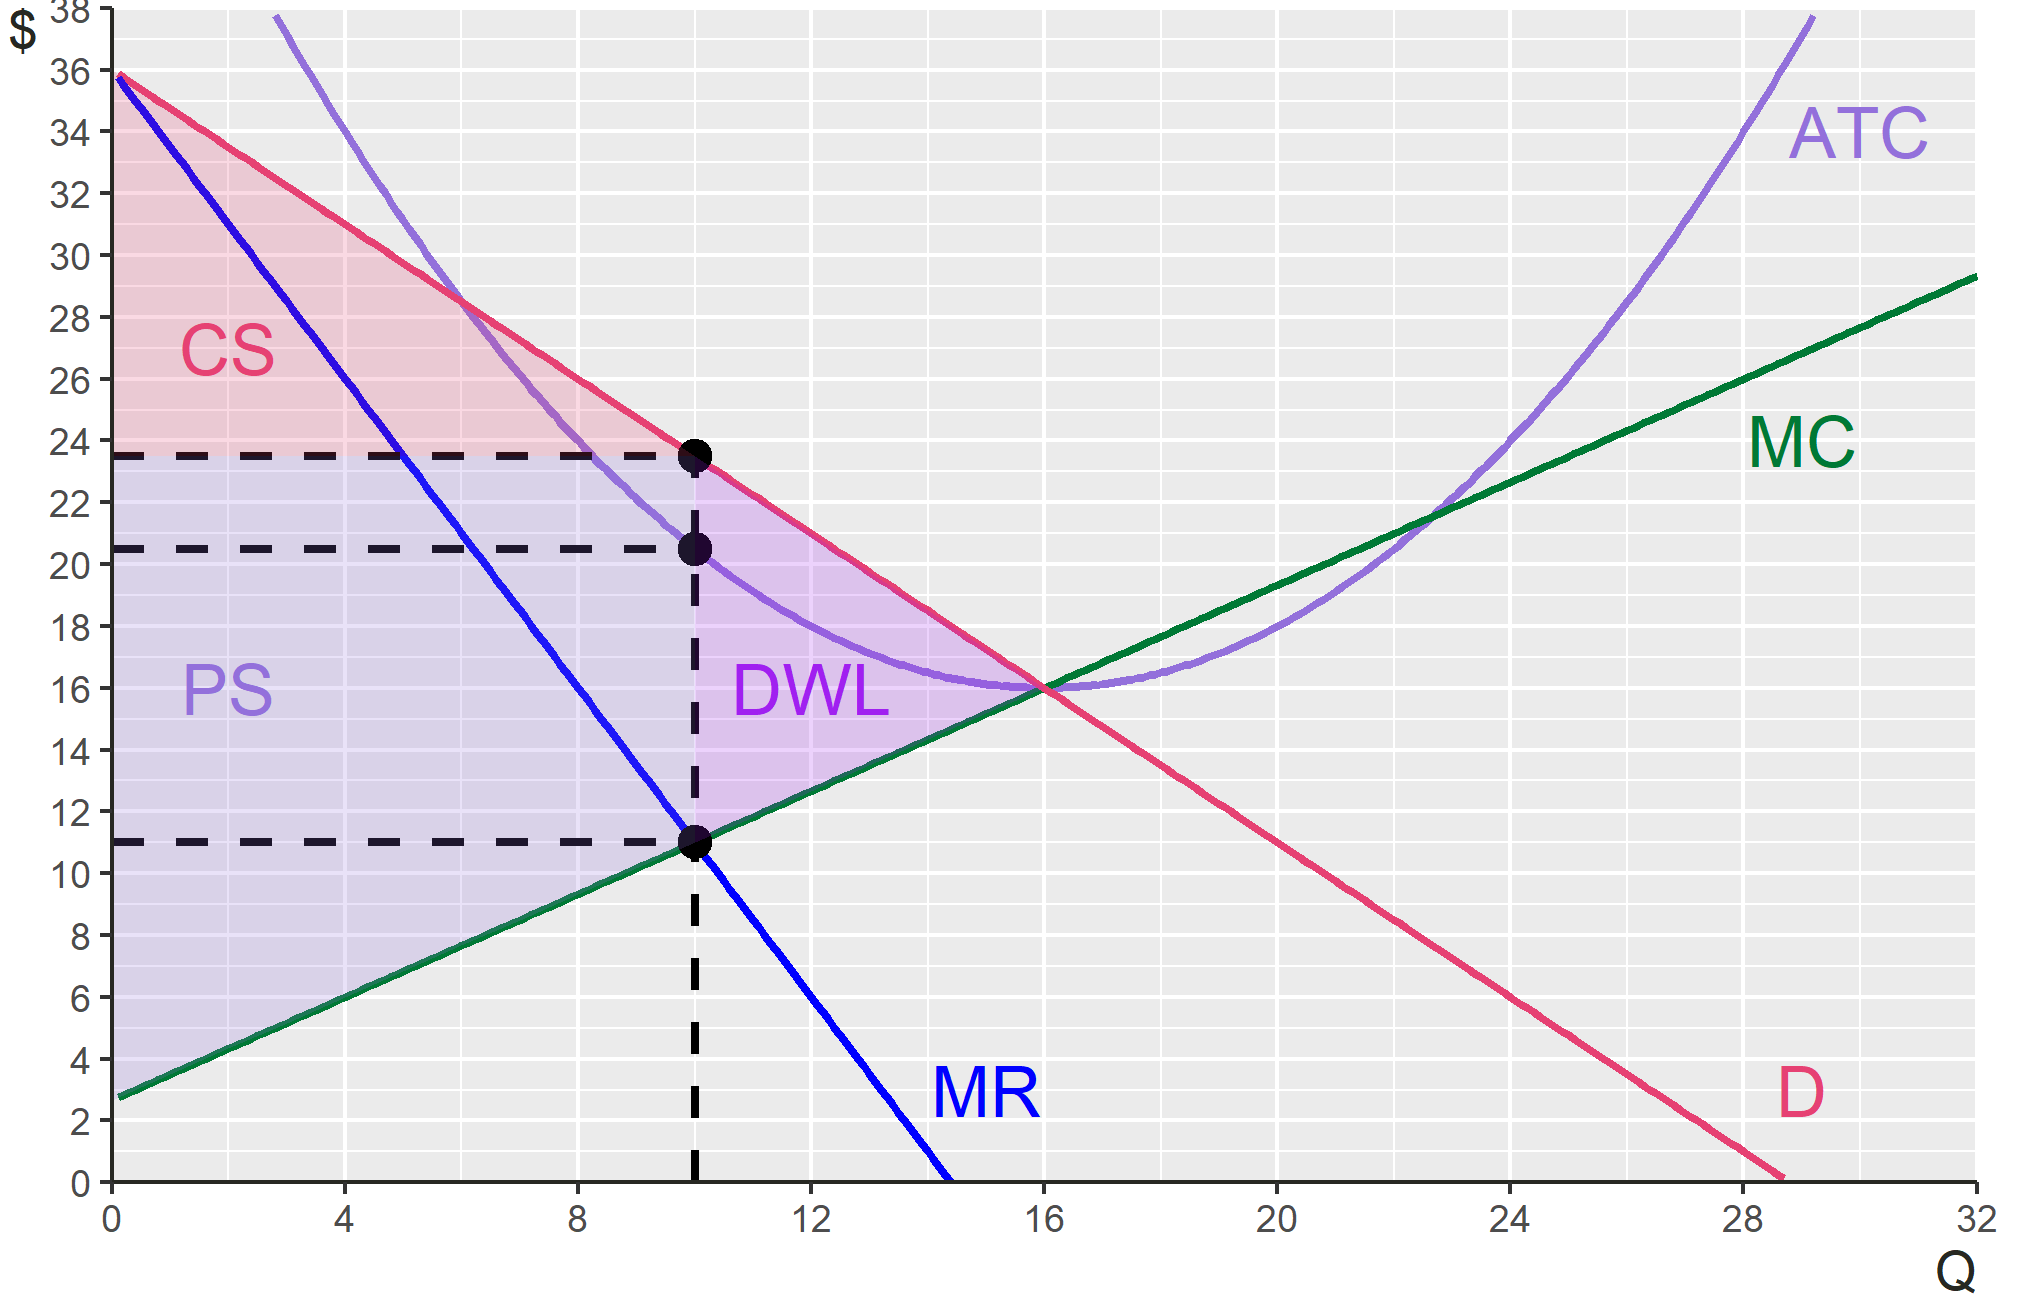
\includegraphics[width=8cm]{pcm 7.png}
			%\caption*{}
		\end{figure}
	\end{itemize}
\end{frame}

\begin{frame}{Summary of Monopoly vs PC}
	\begin{itemize}[<+->]
		\item Under both monopoly and PC, firms produce at $MR=MC$
		\item However, uniquely under PC, $P=MC$
		\item In the long run, PC firms make 0 profit, while monopolists make positive profit. Both of these facts are due to relative barriers to entry (free entry/exit)
		\item Under a monopoly, firms produce less than the efficient amount and are charged higher, leading to DWL
	\end{itemize}
\end{frame}

\begin{frame}{Bonus Question}
	\begin{itemize}[<+->]
		\item Could a price ceiling eliminate the DWL caused by a monopoly?
		\begin{figure}
			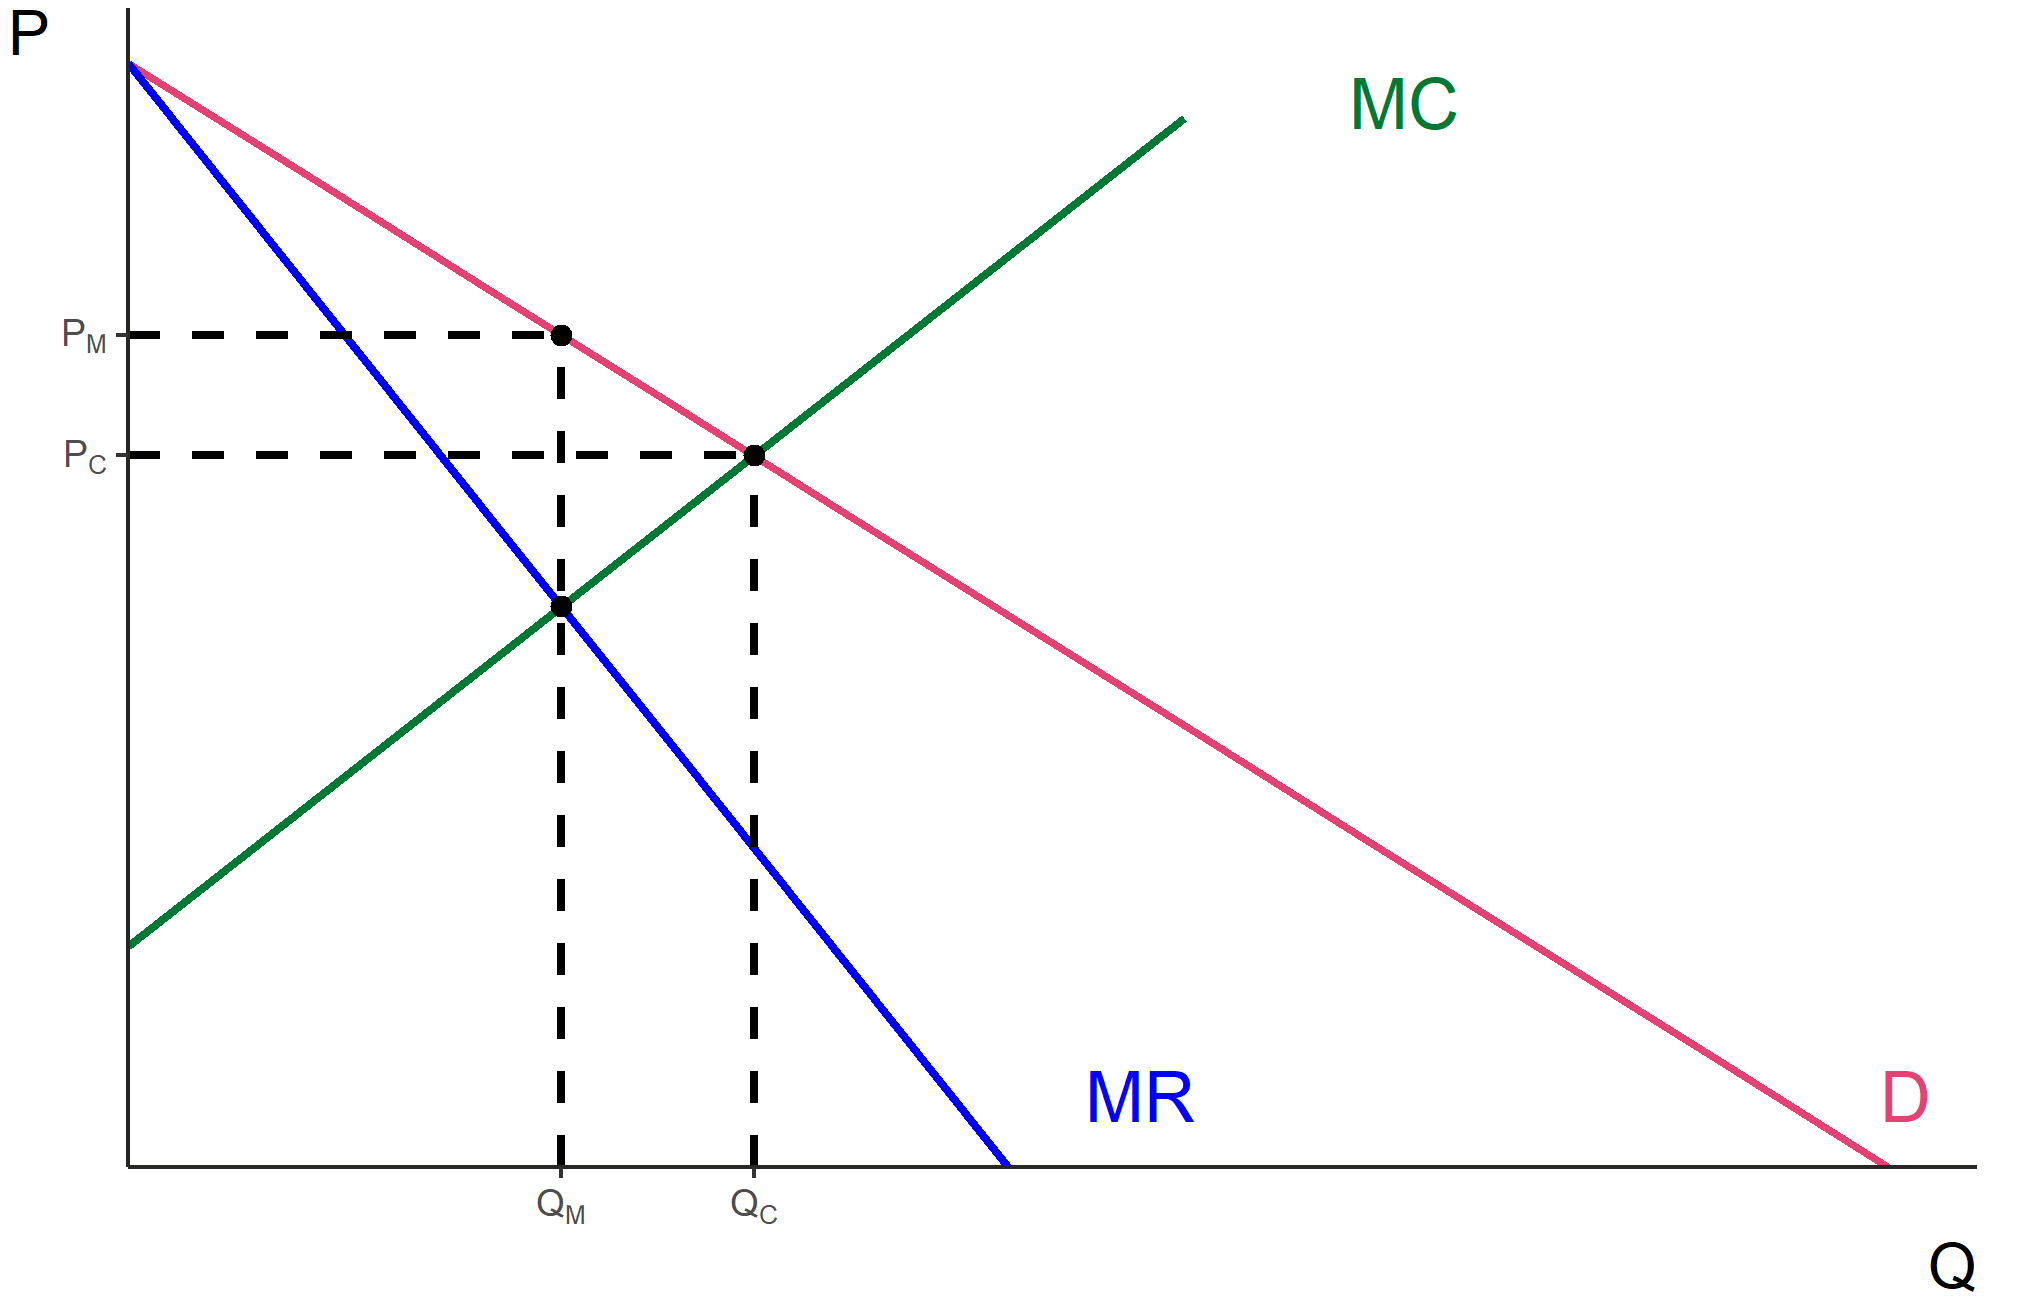
\includegraphics[width=8cm]{price ceil 1.png}
			%\caption*{}
		\end{figure}
	\end{itemize}
\end{frame}

\begin{frame}{Bonus Question}
	\begin{itemize}[<+->]
		\item Recall: the price must be \underline{below} the ceiling
		\begin{figure}
			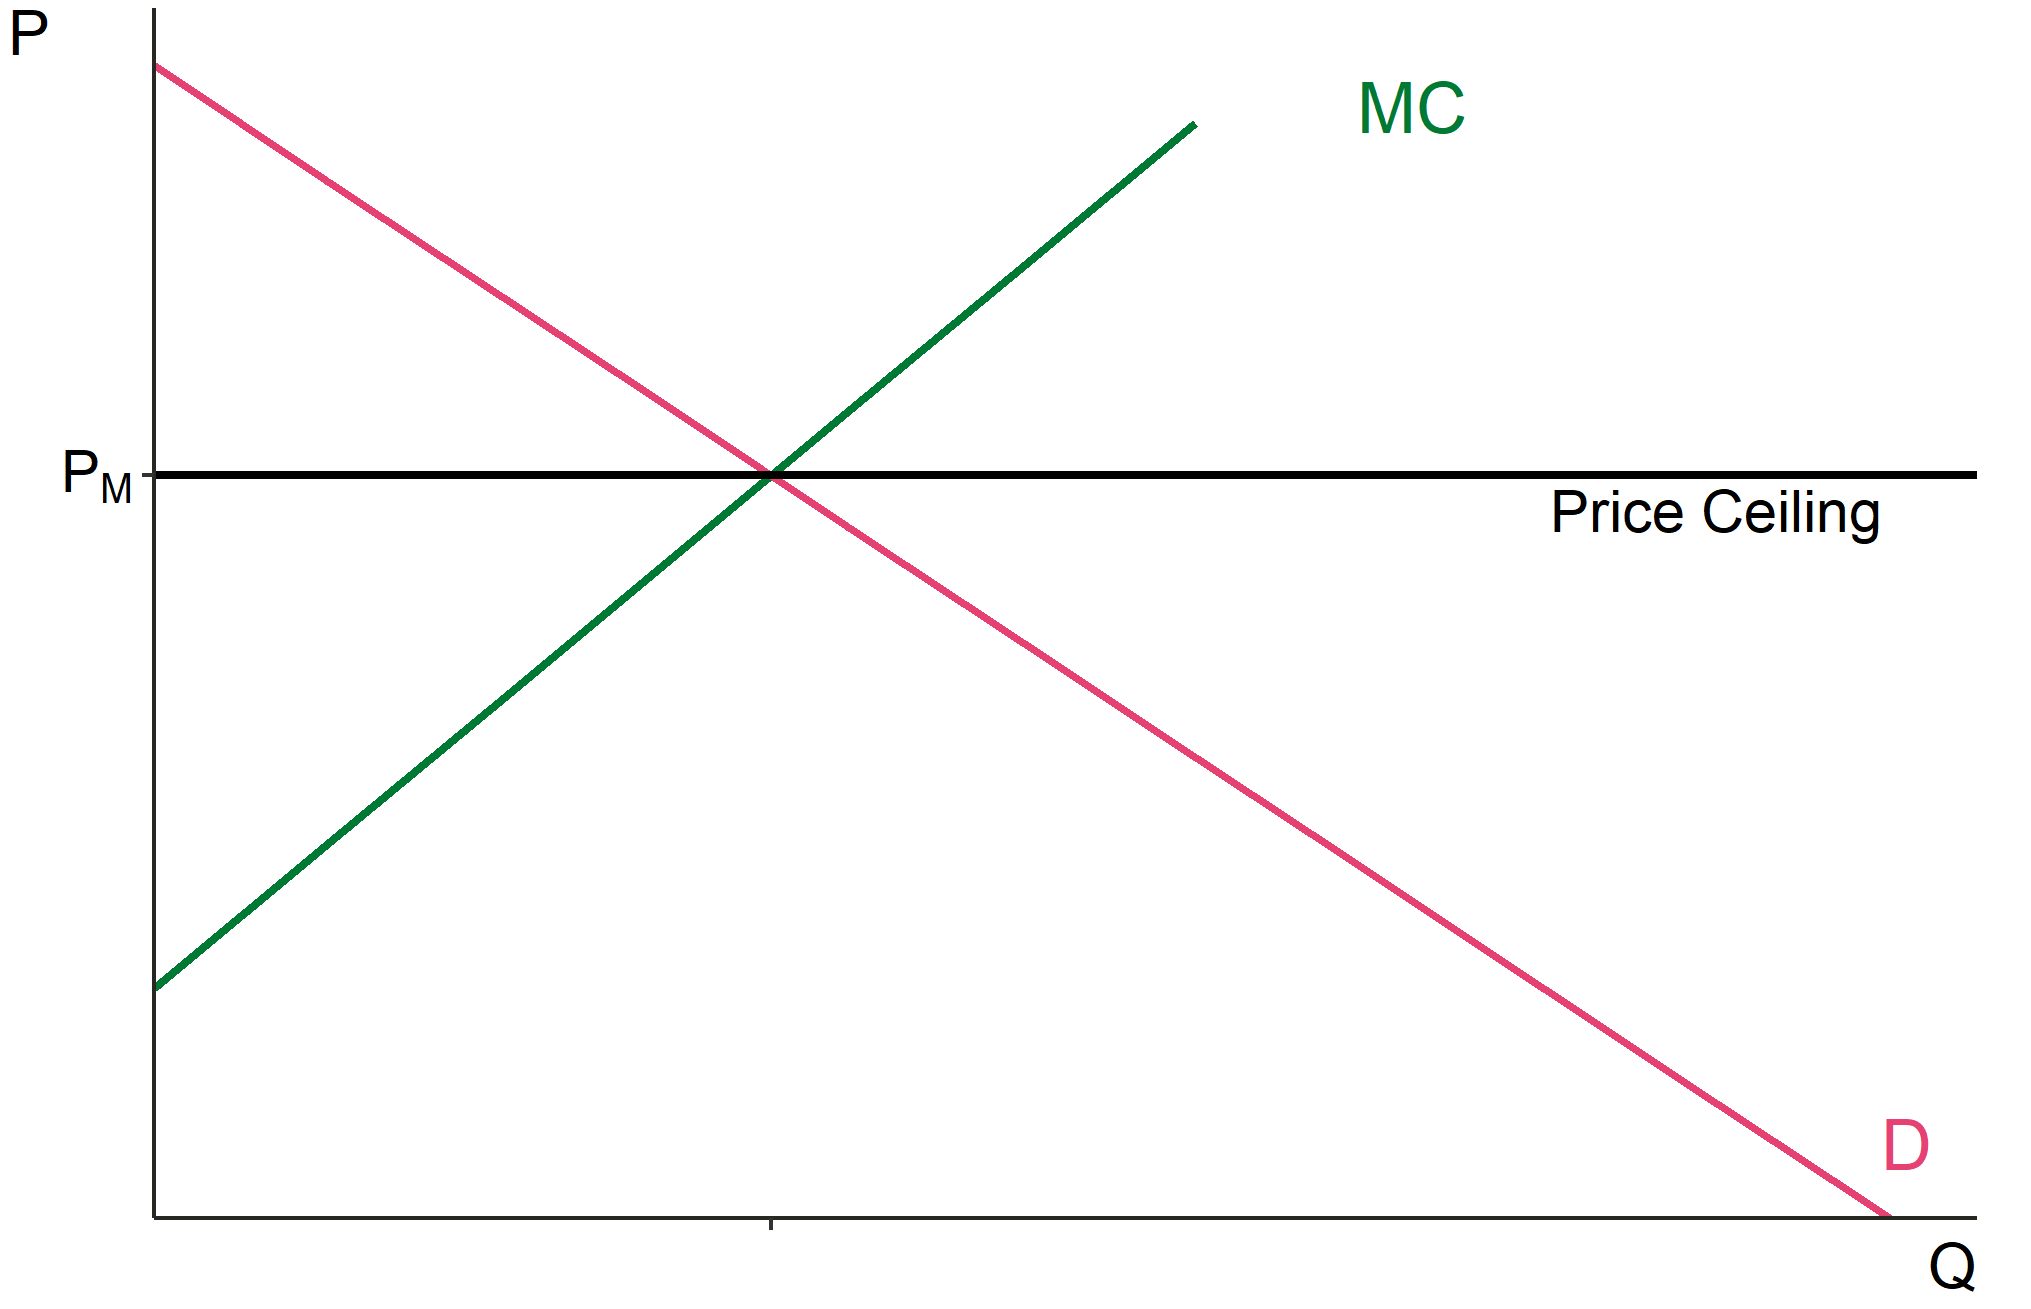
\includegraphics[width=8cm]{price ceil 2.png}
			%\caption*{}
		\end{figure}
		\item What is marginal revenue in this case?
	\end{itemize}
\end{frame}

\begin{frame}{Bonus Question}
	\begin{itemize}[<+->]
		\item So where does the firm produce?
		\begin{figure}
			\includegraphics<1>[width=8cm]{price ceil 3.png}
			\includegraphics<2>[width=8cm]{price ceil 4.png}
			%\caption*{}
		\end{figure}
		\item The firm produces where $MR=MC$, and wants to charge as high of price as possible. So they produce where $MR$ intersects $MC$, and charges at the price ceiling
	\end{itemize}
\end{frame}

\begin{frame}{Bonus Question 1}
	\begin{itemize}[<+->]
		\item So, can a price ceiling eliminate the DWL in a monopoly?
		\begin{figure}
			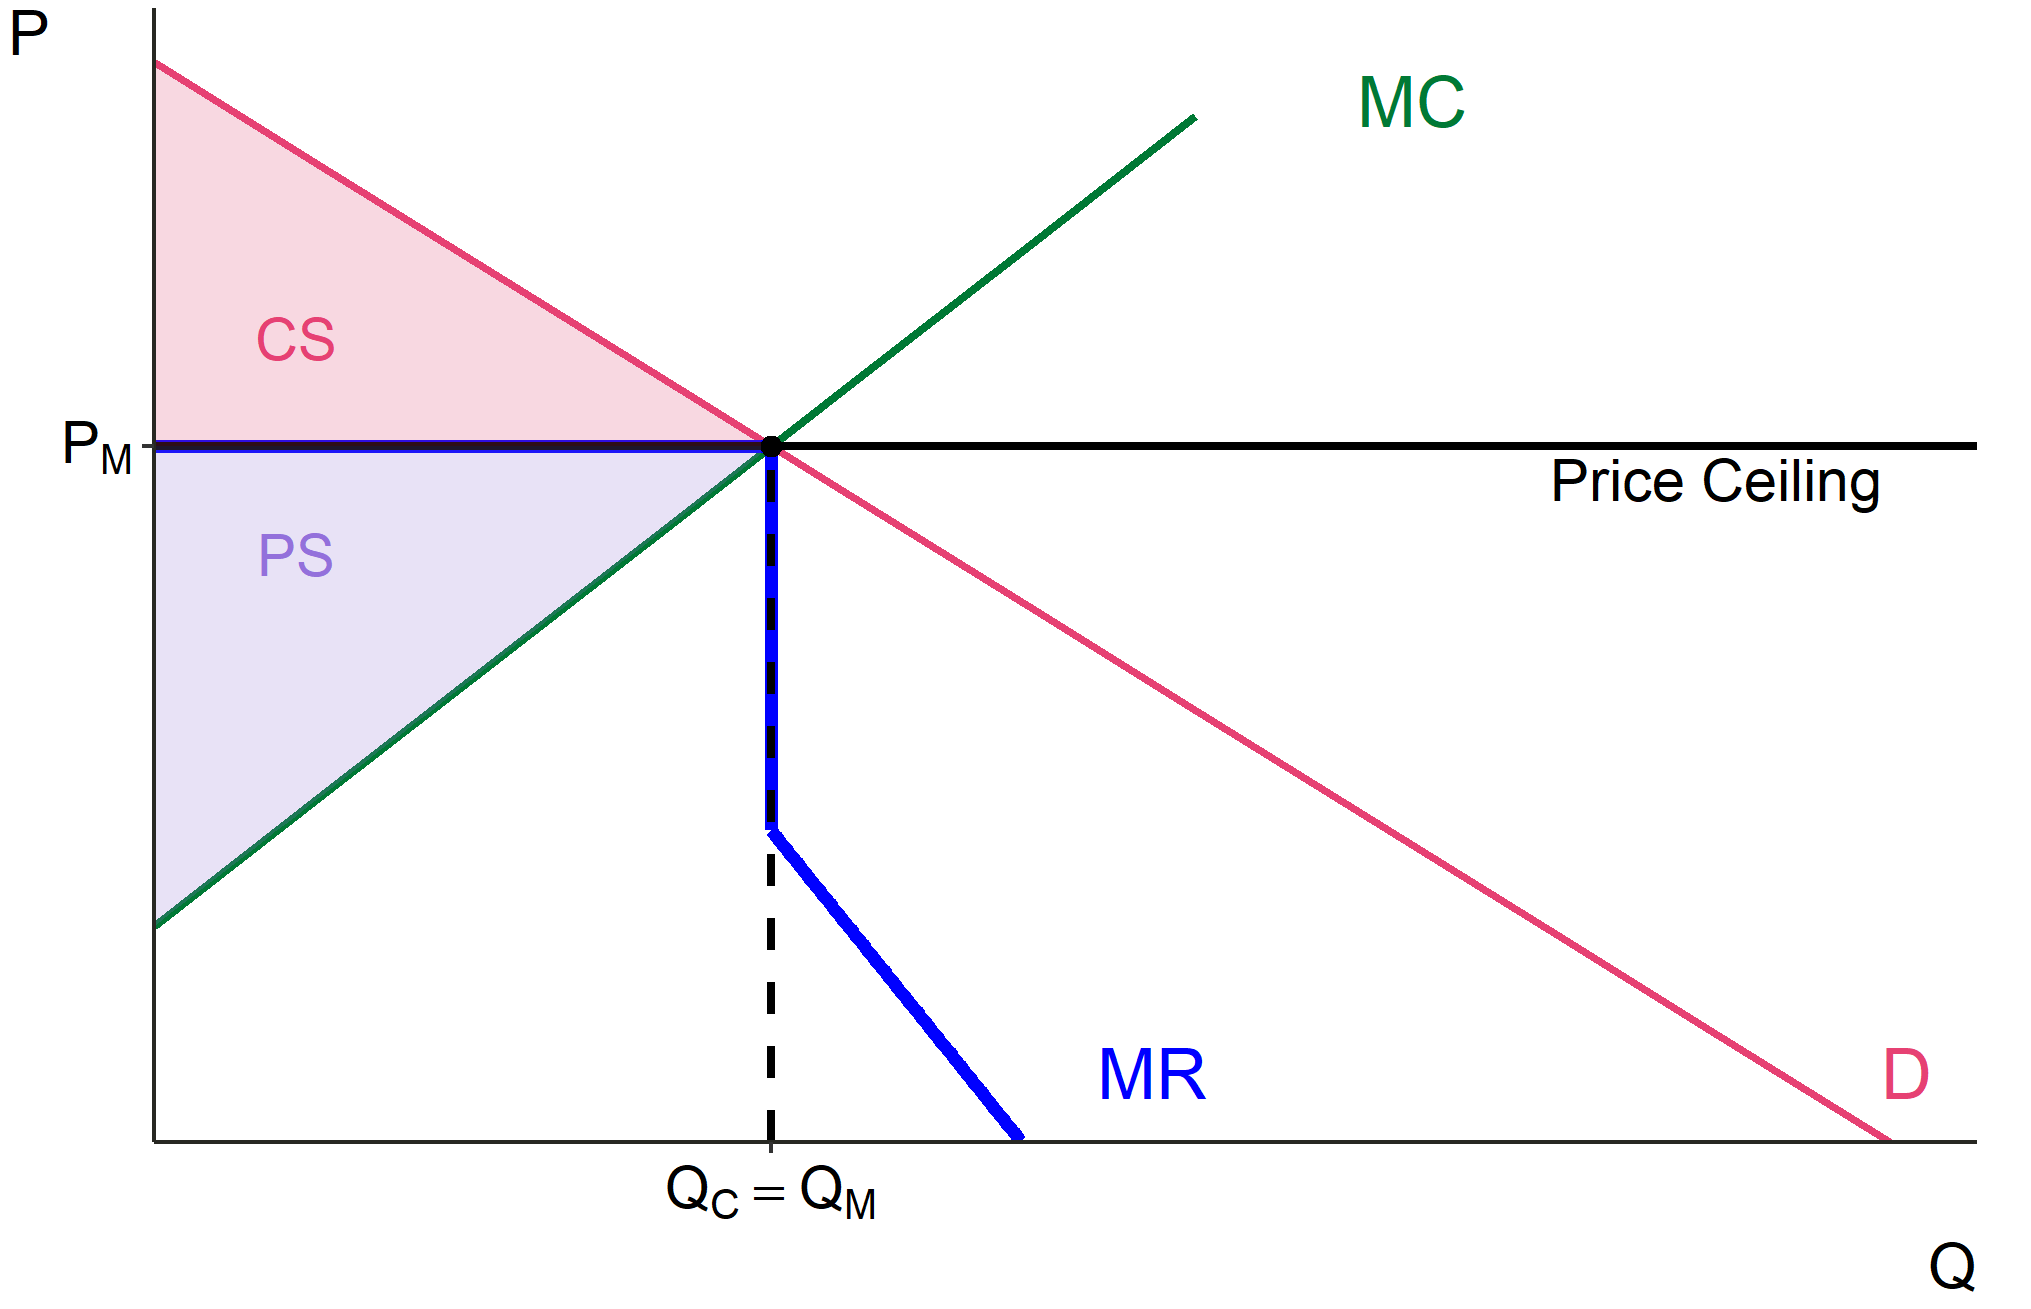
\includegraphics[width=8cm]{price ceil 5.png}
			%\caption*{}
		\end{figure}
		\item A: yes. We are producing at the efficient (competitive) quantity and charging the efficient price
		\begin{itemize}
			\item Can a tax? Think about it.
		\end{itemize}
	\end{itemize}
\end{frame}

\begin{frame}{Summary of Monopolies}
	\begin{itemize}
		\item Read about price discrimination section on your own (15-4b)
		\item Homework 7 due tonight, homework 8 due Monday of Final's week
		\item Wednesday Lecture
		\item Discussion Section this week
		\item Final exam on Thursday, December 9th, at 2:45pm. The exam is 2 hours.
	\end{itemize}
\end{frame}

\end{document}